\documentclass{article}
\usepackage{array}
\usepackage{mathptmx} % Time New Roman
\usepackage{graphicx} % Thư viện chèn ảnh
\usepackage{float} % Set vị trí chèn ảnh
\usepackage{tikz} % Thư viện tạo khung bìa
\usepackage{amssymb} % To use \mathbb
\usepackage{amsmath}
\usepackage{indentfirst} % Thư viện thụt đầu dòng
\usepackage{titlesec} % Thư viện để set up các kiểu chữ
\usepackage{tabularx}
\usepackage{booktabs} % Cho bảng đẹp hơn (toprule, midrule...)
\usepackage{longtable} % Cho bảng dài
\usepackage{lipsum}
\usepackage{colortbl}
\usepackage{forloop}
\usepackage{enumitem}
\usepackage[T5]{fontenc} % Để sử dụng Tiếng Việt
\usepackage[utf8]{inputenc}
\usepackage[font=bf]{caption}
\usepackage[fontsize=13pt]{scrextend} % Set fontsize=13pt
\usepackage[hidelinks,hypertexnames=false]{hyperref}
\usepackage[paperheight=29.7cm,paperwidth=21cm,right=2cm,left=3cm,top=2cm,bottom=2.5cm]{geometry}% A4, margins

\renewcommand{\baselinestretch}{1.2} % Giãn dòng 1.2
\usetikzlibrary{calc} % Thư viện tikz
\setlength{\parskip}{6pt} % Spacing after
\setlength{\parindent}{1cm} % Set khoảng cách thụt đầu dòng mỗi đoạn
\emergencystretch=2em
\setcounter{secnumdepth}{4} % 4 Heading
\titlespacing*{\section}{0pt}{0pt}{30pt} % Heading 1
\titleformat*{\section}{\fontsize{16pt}{0pt}\selectfont \bfseries \centering}
\titlespacing*{\subsection}{0pt}{6pt}{0pt} % Heading 2
\titleformat*{\subsection}{\fontsize{14pt}{0pt}\selectfont \bfseries}
\titlespacing*{\subsubsection}{0pt}{6pt}{0pt} % Heading 3
\titleformat*{\subsubsection}{\fontsize{13pt}{0pt}\selectfont \bfseries \itshape}
\titlespacing*{\paragraph}{0pt}{0pt}{0pt} % Heading 4
\titleformat*{\paragraph}{\fontsize{13pt}{0pt}\selectfont \itshape}

\renewcommand{\figurename}{\fontsize{12pt}{0pt}\selectfont \bfseries Hình}
\renewcommand{\thefigure}{\thesection.\arabic{figure}}
\captionsetup[figure]{labelsep=space}

\renewcommand{\tablename}{\fontsize{12pt}{0pt}\selectfont \bfseries Bảng}
\renewcommand{\thetable}{\thesection.\arabic{table}}
\captionsetup[table]{labelsep=space}

% Định nghĩa lại column types cho tabularx nếu cần
\newcolumntype{s}{>{\hsize=.3\hsize}X}
\newcolumntype{y}{>{\hsize=.4\hsize}X}
\newcolumntype{d}{>{\hsize=.1\hsize}X}
\newcolumntype{a}{>{\hsize=1.1\hsize}X}
\newcolumntype{g}{>{\hsize=5\hsize}X}
\renewcommand{\tabularxcolumn}[1]{>{\small}m{#1}}

\renewcommand{\theequation}{\thesection.\arabic{equation}}
\newtheorem{theorem}{Định lý}[section]
\newtheorem{defn}[theorem]{Định nghĩa}
\newtheorem{corollary}[theorem]{Hệ quả}
\newtheorem{lemma}[theorem]{Bổ đề}

\renewcommand{\contentsname}{MỤC LỤC}
\renewcommand{\listfigurename}{DANH MỤC HÌNH VẼ}
\renewcommand{\listtablename}{DANH MỤC BẢNG BIỂU}
\renewcommand{\refname}{TÀI LIỆU THAM KHẢO}


\definecolor{LightCyan}{rgb}{0.88,1,1}
\newcounter{loopcntr}
\newcommand{\rpt}[2][1]{\forloop{loopcntr}{0}{\value{loopcntr}<#1}{#2}}

\setitemize{itemsep=0pt,leftmargin=1.25cm,topsep = 3pt}

\begin{document}

\begin{titlepage}
    \begin{tikzpicture}[overlay,remember picture]
        \draw [line width=3pt]
        ($ (current page.north west) + (3.0cm,-2.0cm) $)
        rectangle
        ($ (current page.south east) + (-2.0cm,2.5cm) $);
        \draw [line width=0.5pt]
        ($ (current page.north west) + (3.1cm,-2.1cm) $)
        rectangle
        ($ (current page.south east) + (-2.1cm,2.6cm) $);
    \end{tikzpicture}
    \begin{center}
        \vspace{-12pt}  ĐẠI HỌC QUỐC GIA THÀNH PHỐ HỒ CHÍ MINH\\
        \textbf{\fontsize{16pt}{0pt}\selectfont TRƯỜNG ĐẠI HỌC KHOA HỌC TỰ NHIÊN}
        \vspace{0.5cm}
        \begin{figure}[H]
            \centering
            
\includegraphics[width=2.26cm,height=2.26cm]{outputs/logo.png}
        \end{figure}
        \vspace{1.5cm}
        \fontsize{24pt}{0pt}\selectfont BÁO CÁO CUỐI KÌ\\
        \vspace{12pt}
        \textbf{\fontsize{32pt}{0pt}\selectfont XỬ LÝ SỐ LIỆU THỐNG KÊ}
        \vspace{1.5cm}
    \end{center}
    \begin{center}
        \hspace{6pt}\textbf{\fontsize{14pt}{0pt}\selectfont ĐỀ TÀI:}
    \end{center}
    \begin{center}
        \textbf{\fontsize{20pt}{0pt}\selectfont PHÂN TÍCH VÀ DỰ ĐOÁN NGUY CƠ TIỂU ĐƯỜNG TỪ DỮ LIỆU BRFSS 2015}
        \vspace{1.5cm}
        \begin{table}[H]
            \centering
            \begin{tabular}{l l}
                \fontsize{14pt}{0pt}\selectfont Giảng viên:     & \fontsize{14pt}{0pt}\selectfont Thầy Tô Đức Khánh \\[6pt]
                \fontsize{14pt}{0pt}\selectfont Nhóm thực hiện: & \fontsize{14pt}{0pt}\selectfont Nhóm C            \\[6pt]
                \fontsize{14pt}{0pt}\selectfont Sinh viên:      & \fontsize{14pt}{0pt}\selectfont Nguyễn Đức Mạnh   \\[6pt]
                \fontsize{14pt}{0pt}\selectfont MSSV:           & \fontsize{14pt}{0pt}\selectfont 20280065          \\[6pt]
            \end{tabular}

        \end{table}
        \vspace{2cm}
        \fontsize{14pt}{0pt}\selectfont TP. Hồ Chí Minh - \the\year
    \end{center}
\end{titlepage}
\newpage

% Mục lục
\addtocontents{toc}{\protect\thispagestyle{empty}}
\tableofcontents
\thispagestyle{empty}
\cleardoublepage

% Danh mục bảng
\phantomsection
\addcontentsline{toc}{section}{\numberline{}DANH MỤC BẢNG BIỂU}
{\let\oldnumberline\numberline
    \renewcommand{\numberline}{Bảng~\oldnumberline}
    \listoftables}
\newpage

% Danh mục hình
\phantomsection
\addcontentsline{toc}{section}{\numberline{}DANH MỤC HÌNH VẼ}
{\let\oldnumberline\numberline
    \renewcommand{\numberline}{Hình~\oldnumberline}
    \listoffigures}
\newpage

% -----------------------------------------------------------------------------
% LỜI NÓI ĐẦU
% -----------------------------------------------------------------------------
\section*{LỜI NÓI ĐẦU}
\thispagestyle{empty}
Bệnh tiểu đường hiện nay đang là một vấn đề sức khỏe cộng đồng nghiêm trọng, ảnh hưởng lớn đến chất lượng cuộc sống và tuổi thọ. Trong bối cảnh khoa học dữ liệu ngày càng phát triển, việc ứng dụng các kỹ thuật phân tích và học máy để dự đoán sớm nguy cơ mắc bệnh là một hướng đi thiết thực và có ý nghĩa.

Trong đồ án này, em đã thực hiện quy trình phân tích dữ liệu trên bộ BRFSS 2015. Quá trình thực hiện bao gồm các bước từ tiền xử lý, làm sạch dữ liệu, phân tích khám phá (EDA) đến việc xây dựng và đánh giá các mô hình học máy. Đặc biệt, vấn đề mất cân bằng dữ liệu (imbalanced data) đã được chú trọng xử lý để nâng cao hiệu quả dự báo.

Báo cáo chắc chắn không tránh khỏi những thiếu sót, em rất mong nhận được sự góp ý của Thầy để có thể hoàn thiện hơn.
\cleardoublepage

% -----------------------------------------------------------------------------
% TÓM TẮT ĐỒ ÁN
% -----------------------------------------------------------------------------
\section*{TÓM TẮT ĐỒ ÁN}
\phantomsection\addcontentsline{toc}{section}{\numberline {}TÓM TẮT ĐỒ ÁN}
Đồ án này tập trung nghiên cứu các yếu tố nguy cơ dẫn đến bệnh tiểu đường dựa trên bộ dữ liệu BRFSS 2015, đồng thời xây dựng và đánh giá hiệu quả của các mô hình học máy trong việc dự đoán nguy cơ mắc bệnh.

Các kết quả chính đạt được:
\begin{itemize}
    \item Xác định các yếu tố có ảnh hưởng đáng kể nhất: \textbf{Huyết áp cao (HighBP)} và \textbf{Khó khăn khi đi lại (DiffWalk)} là những chỉ báo quan trọng nhất với mức độ ảnh hưởng (Effect Size) cao nhất.
    \item Chỉ số khối cơ thể (BMI) cho thấy xu hướng tăng rõ rệt theo mức độ nghiêm trọng của bệnh (trung bình 27.7 ở người khỏe mạnh so với 31.9 ở người bệnh).
    \item Về mô hình dự đoán: Do dữ liệu mất cân bằng nặng, các mô hình cơ bản (Baseline) không hiệu quả. Việc áp dụng chiến lược **Random Under-sampling** kết hợp với **Naive Bayes** cho kết quả F1-score ổn định nhất trên tập kiểm tra (khoảng \textbf{0.66}) cho bài toán phân loại nhị phân.
    \item Chiến lược gán trọng số (Class Weight) với Logistic Regression giúp cải thiện đáng kể chỉ số Balanced Accuracy (đạt khoảng \textbf{0.74}), giúp mô hình không bị thiên lệch về nhóm đa số.
\end{itemize}
\cleardoublepage

\pagenumbering{roman}

% -----------------------------------------------------------------------------
% DANH MỤC KÝ HIỆU
% -----------------------------------------------------------------------------
\section*{DANH MỤC KÝ HIỆU VÀ CHỮ VIẾT TẮT}
\phantomsection \addcontentsline{toc}{section}{\numberline {} DANH MỤC KÝ HIỆU VÀ CHỮ VIẾT TẮT}

\noindent
\begin{tabularx}{\textwidth}{ l X }
    \hspace{1cm} \textbf{Từ viết tắt} & \textbf{Giải thích}                                    \\
    \hspace{1cm} BRFSS                & Behavioral Risk Factor Surveillance System             \\
    \hspace{1cm} EDA                  & Exploratory Data Analysis (Phân tích khám phá dữ liệu) \\
    \hspace{1cm} BMI                  & Body Mass Index (Chỉ số khối cơ thể)                   \\
    \hspace{1cm} CV                   & Cross-Validation (Kiểm định chéo)                      \\
    \hspace{1cm} AUC                  & Area Under the Curve                                   \\
    \hspace{1cm} ROC                  & Receiver Operating Characteristic                      \\
    \hspace{1cm} OR                   & Odds Ratio (Tỷ số chênh)                               \\
\end{tabularx}

\newpage
\pagenumbering{arabic}

% =============================================================================
% A. ĐỀ TÀI
% =============================================================================
\section{A. ĐỀ TÀI}

Hiện nay, bệnh tiểu đường là một căn bệnh mãn tính phổ biến nhất trên thế giới. Bệnh tiểu đường là một căn bệnh mãn tính nghiêm trọng khiến mọi người mất khả năng điều chỉnh hiệu quả lượng glucose trong máu và có thể dẫn đến giảm chất lượng cuộc sống và tuổi thọ. Các biến chứng như bệnh tim, mất thị lực, cắt cụt chi dưới và bệnh thận có liên quan đến lượng đường cao mãn tính vẫn còn trong máu đối với những người mắc bệnh tiểu đường.

Mặc dù không có cách chữa khỏi bệnh tiểu đường, nhưng các chiến lược như giảm cân, ăn uống lành mạnh, vận động và điều trị y tế có thể làm giảm tác hại của căn bệnh này ở nhiều bệnh nhân. Chẩn đoán sớm có thể dẫn đến thay đổi lối sống và điều trị hiệu quả hơn, khiến các mô hình dự đoán nguy cơ mắc bệnh tiểu đường trở thành công cụ quan trọng đối với cộng đồng và các quan chức y tế công cộng.

Dữ liệu \texttt{diabetes\_012\_health\_indicators\_BRFSS2015.csv} chứa thông tin khảo sát của 253,680 người dân Hoa Kỳ (năm 2015), với 22 biến được quan sát. Dưới đây là mô tả sơ bộ về các biến mà em đã tìm hiểu:

\begin{itemize}
    \item \textbf{Diabetes\_012}: Tình trạng bệnh (0: không, 1: tiền tiểu đường, 2: tiểu đường).
    \item \textbf{HighBP}: Cao huyết áp (0/1).
    \item \textbf{HighChol}: Cholesterol cao (0/1).
    \item \textbf{CholCheck}: Đã kiểm tra cholesterol trong 5 năm (0/1).
    \item \textbf{BMI}: Chỉ số khối cơ thể.
    \item \textbf{Smoker}: Đã hút ít nhất 100 điếu thuốc trong đời (0/1).
    \item \textbf{Stroke}: Đã từng đột quỵ (0/1).
    \item \textbf{HeartDiseaseorAttack}: Bệnh tim mạch vành hoặc nhồi máu cơ tim (0/1).
    \item \textbf{PhysActivity}: Hoạt động thể chất trong 30 ngày (0/1).
    \item \textbf{Sex}: Giới tính (0: Nữ, 1: Nam).
    \item \textbf{Age}: Nhóm tuổi (13 mức).
    \item \textbf{Education}: Trình độ học vấn (1-6).
    \item \textbf{Income}: Mức thu nhập (1-8).
    \item \textbf{GenHlth}: Sức khỏe tự đánh giá (1-5).
    \item Và một số biến khác...
\end{itemize}

% =============================================================================
% B. YÊU CẦU
% =============================================================================
\newpage
\section{B. YÊU CẦU}

Để hoàn thành đồ án này, các yêu cầu sau đã được bám sát:

\subsection{1. Bản đề xuất \& 2. Mục tiêu phân tích}
Mục tiêu của đồ án bao gồm:
\begin{enumerate}
    \item \textbf{Mục tiêu 1 (M1)}: Phân tích sự phân bố của dữ liệu, đặc biệt là tình trạng mất cân bằng giữa các nhóm (người bệnh và người khỏe mạnh).
    \item \textbf{Mục tiêu 2 (M2)}: Xác định các yếu tố nguy cơ quan trọng nhất ảnh hưởng đến bệnh tiểu đường.
    \item \textbf{Mục tiêu 3 (M3)}: Xây dựng các mô hình học máy để dự đoán nguy cơ mắc bệnh dựa trên các chỉ số sức khỏe.
    \item \textbf{Mục tiêu 4 (M4)}: Tối ưu hóa mô hình để đạt được độ chính xác và hiệu quả cao nhất, đặc biệt trong việc nhận diện các trường hợp mắc bệnh.
\end{enumerate}

\subsection{3. Phương pháp và chiến lược}
Quy trình thực hiện bao gồm các bước:
\begin{itemize}
    \item \textbf{Bước 1 - Data Ingestion \& QC:} Thu thập, đọc dữ liệu và kiểm tra chất lượng (xử lý giá trị thiếu, dữ liệu nhiễu).
    \item \textbf{Bước 2 - Define Cases:} Phân chia bài toán thành các trường hợp cụ thể (Case A, B, C) để thuận tiện cho việc thử nghiệm và đánh giá.
    \item \textbf{Bước 3 - EDA:} Thực hiện phân tích khám phá dữ liệu thông qua biểu đồ và các chỉ số thống kê mô tả.
    \item \textbf{Bước 4 - Statistical Tests:} Sử dụng các kiểm định thống kê (Chi-square, Kruskal-Wallis) để sàng lọc và lựa chọn biến quan trọng.
    \item \textbf{Bước 5 - Modeling:} Huấn luyện các mô hình học máy (Logistic Regression, Naive Bayes...) kết hợp với các kỹ thuật xử lý mất cân bằng dữ liệu (SMOTE, Class Weight).
    \item \textbf{Bước 6 - Evaluation:} Đánh giá hiệu năng mô hình dựa trên các chỉ số như F1-score và ROC/AUC.
\end{itemize}

\subsection{4. Mô tả và biểu diễn tổng hợp dữ liệu}
Dưới đây là các bảng và biểu đồ tổng hợp từ dữ liệu gốc.

Đầu tiên, phân bố số lượng mẫu ở các trường hợp (Cases) cho thấy sự chênh lệch lớn. Cụ thể ở \textbf{Case A} (3 lớp), nhóm người khỏe mạnh chiếm tới \textbf{84.2\%}, trong khi nhóm tiền tiểu đường chỉ chiếm vỏn vẹn \textbf{1.8\%}, tạo ra tỷ lệ mất cân bằng (Imbalance Ratio) lên tới \textbf{46.15}. Ngay cả khi gộp nhóm (Case B), tỷ lệ chênh lệch vẫn ở mức cao (6.18).

\begin{table}[H]
    \centering
    \caption{Phân bố biến mục tiêu và các Cases}
    
\begin{tabular}{lrrlr}
\toprule
Class & Count & Proportion & Case & ImbalanceRatio\\
\midrule
0 & 213703 & 0.8424117 & CaseA & 46.15\\
1 & 4631 & 0.0182553 & CaseA & 46.15\\
2 & 35346 & 0.1393330 & CaseA & 46.15\\
0 & 218334 & 0.8606670 & CaseB & 6.18\\
1 & 35346 & 0.1393330 & CaseB & 6.18\\
\addlinespace
0 & 213703 & 0.8424117 & CaseC & 5.35\\
1 & 39977 & 0.1575883 & CaseC & 5.35\\
\bottomrule
\end{tabular}

\end{table}

Về các chỉ số sức khỏe, sự phân hóa thể hiện rõ nét nhất qua chỉ số BMI. Biểu đồ dưới đây và bảng thống kê cho thấy: BMI trung bình tăng dần từ nhóm Khỏe mạnh (\textbf{27.7}) lên nhóm Tiền tiểu đường (\textbf{30.7}) và cao nhất ở nhóm Tiểu đường (\textbf{31.9}). Điều này củng cố giả thuyết béo phì là yếu tố nguy cơ lớn.

\begin{figure}[H]
    \centering
    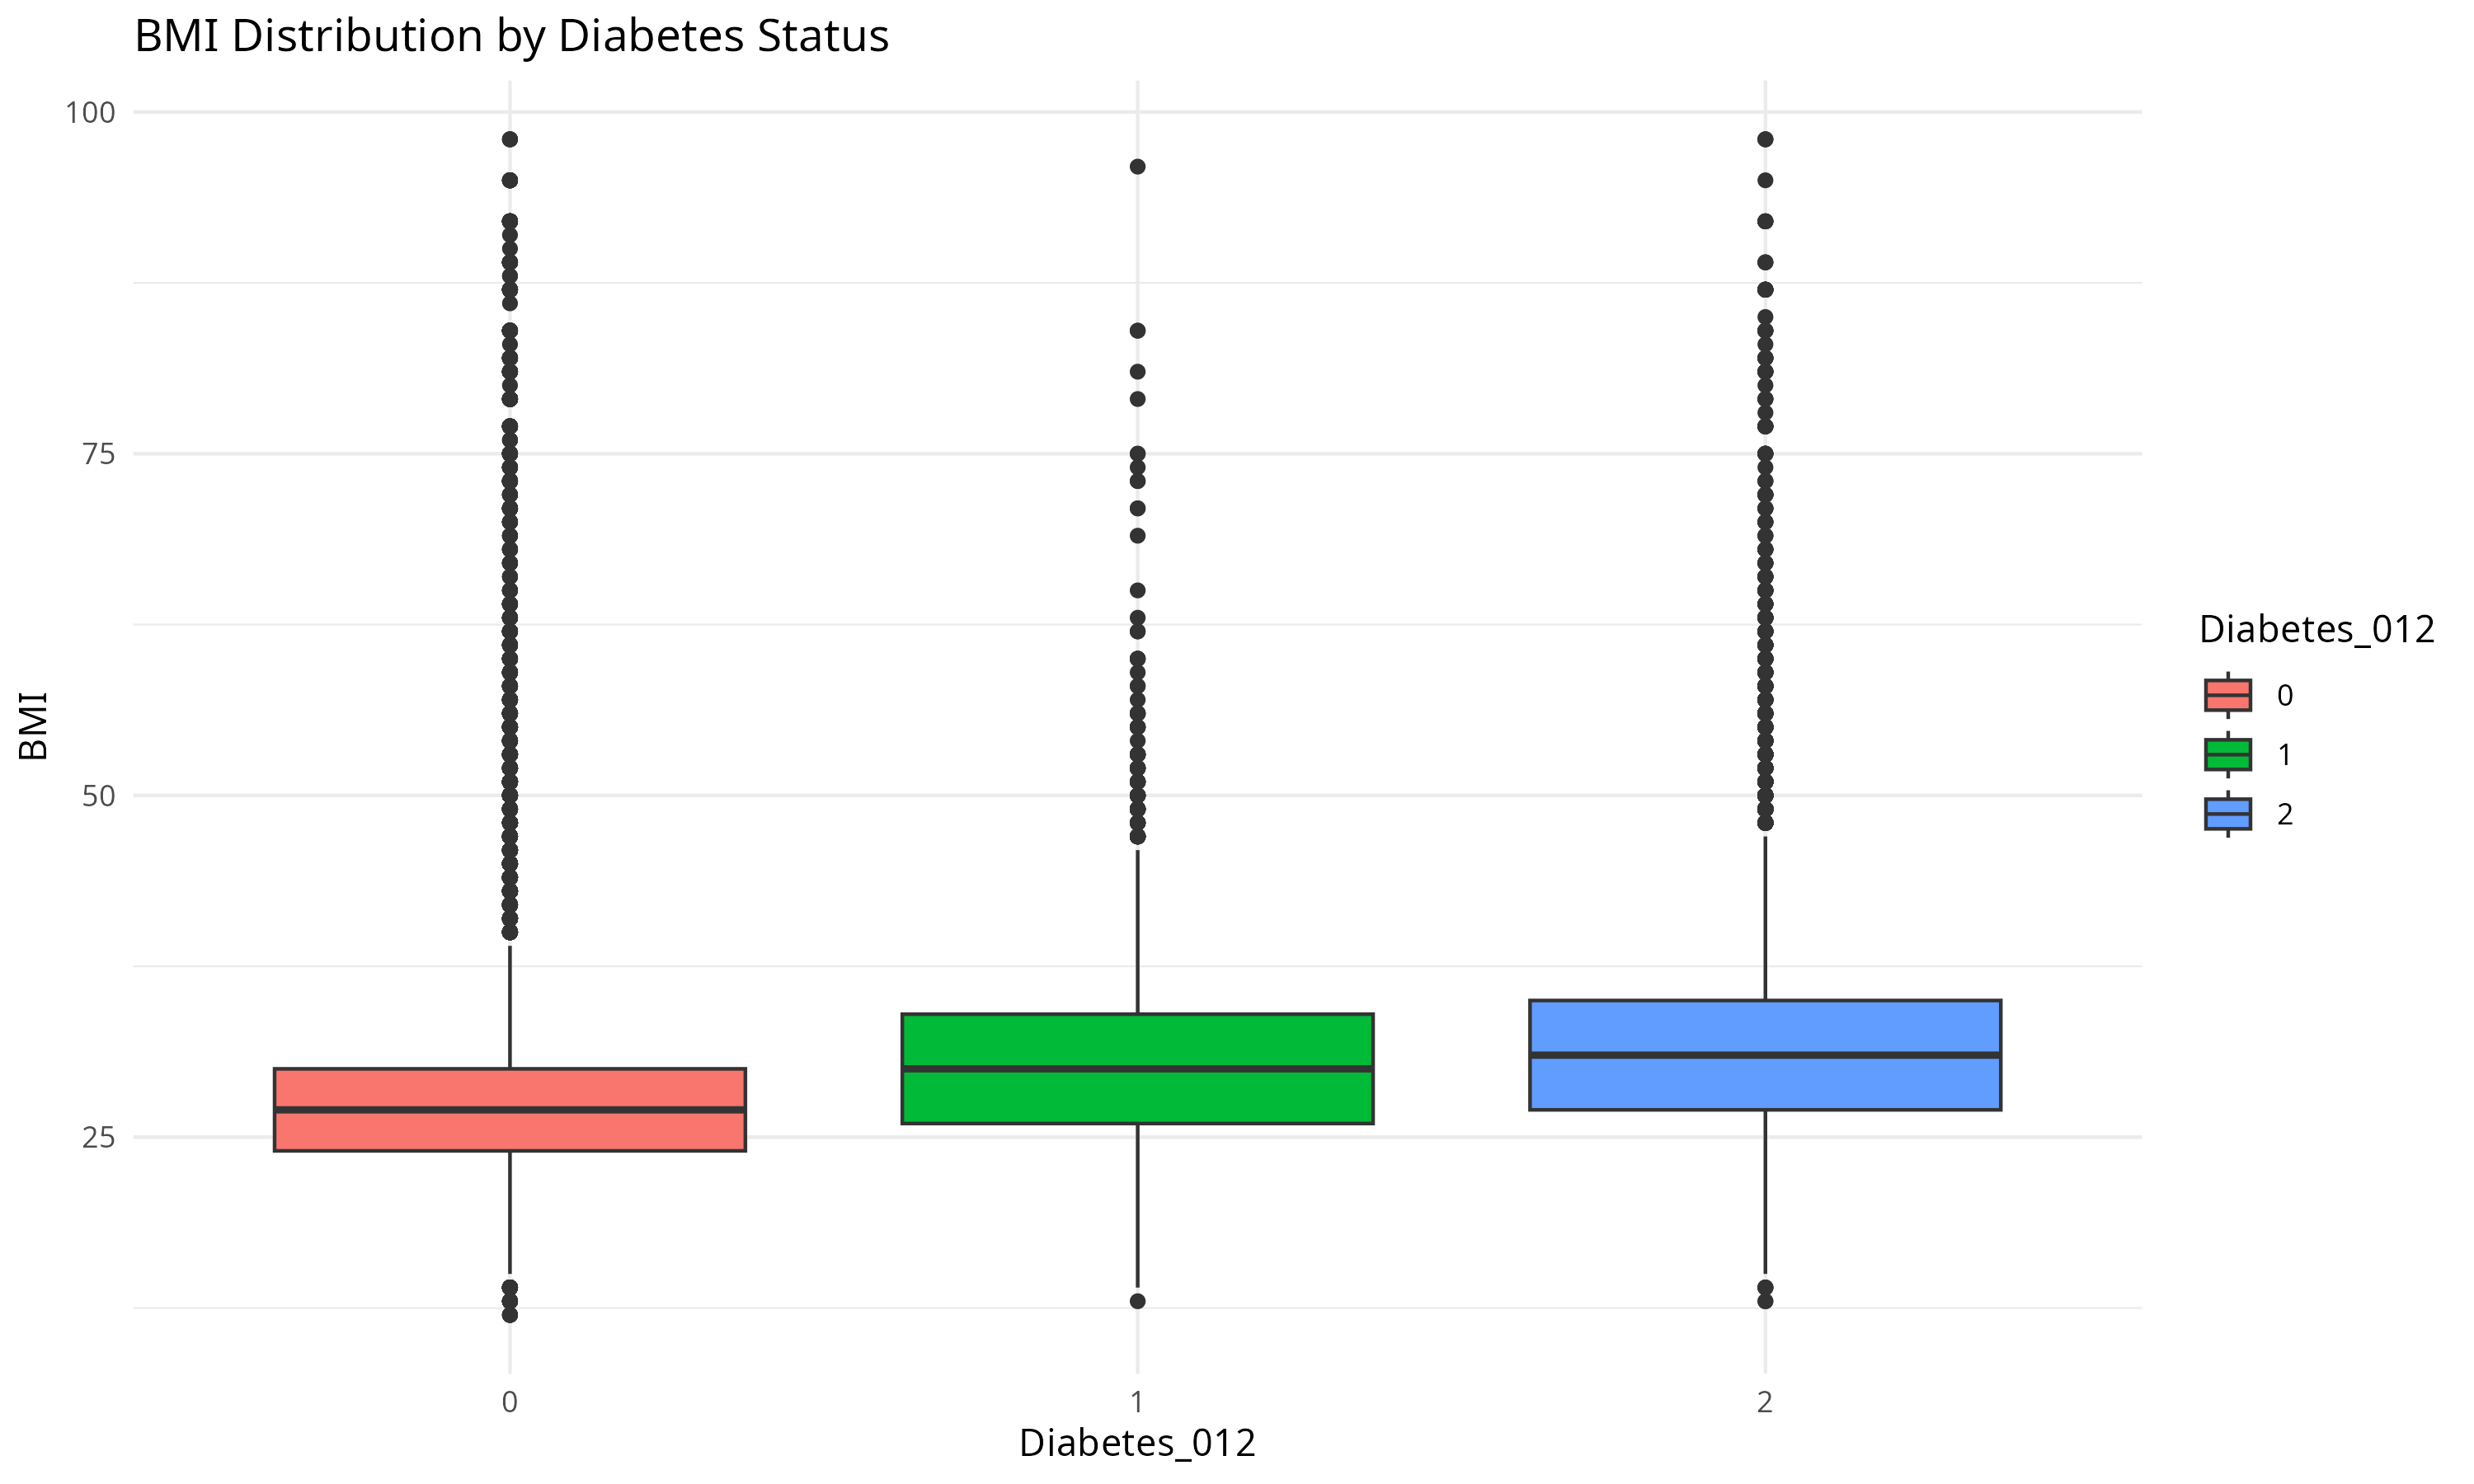
\includegraphics[width=0.8\textwidth]{outputs/figures/F1_bmi_boxplot.png}
    \caption{Phân bố BMI theo tình trạng bệnh}
\end{figure}

Bảng thống kê chi tiết cho thấy không chỉ BMI, mà số ngày sức khỏe tâm thần (MentHlth) và thể chất (PhysHlth) kém cũng cao hơn hẳn ở nhóm bệnh:
\begin{table}[H]
    \centering
    \caption{Thống kê mô tả các biến số thực}
    \resizebox{\textwidth}{!}{
        
\begin{tabular}{lrrrrrrrrr}
\toprule
Diabetes\_012 & BMI\_mean & BMI\_sd & BMI\_median & MentHlth\_mean & MentHlth\_sd & MentHlth\_median & PhysHlth\_mean & PhysHlth\_sd & PhysHlth\_median\\
\midrule
0 & 27.74252 & 6.260993 & 27 & 2.944404 & 7.064440 & 0 & 3.582416 & 7.999205 & 0\\
1 & 30.72447 & 6.964898 & 30 & 4.529907 & 8.897176 & 0 & 6.348305 & 10.298013 & 0\\
2 & 31.94401 & 7.363401 & 31 & 4.461806 & 8.947717 & 0 & 7.954479 & 11.301490 & 1\\
\bottomrule
\end{tabular}

    }
\end{table}

Về các thói quen và bệnh lý đi kèm:
\begin{figure}[H]
    \centering
    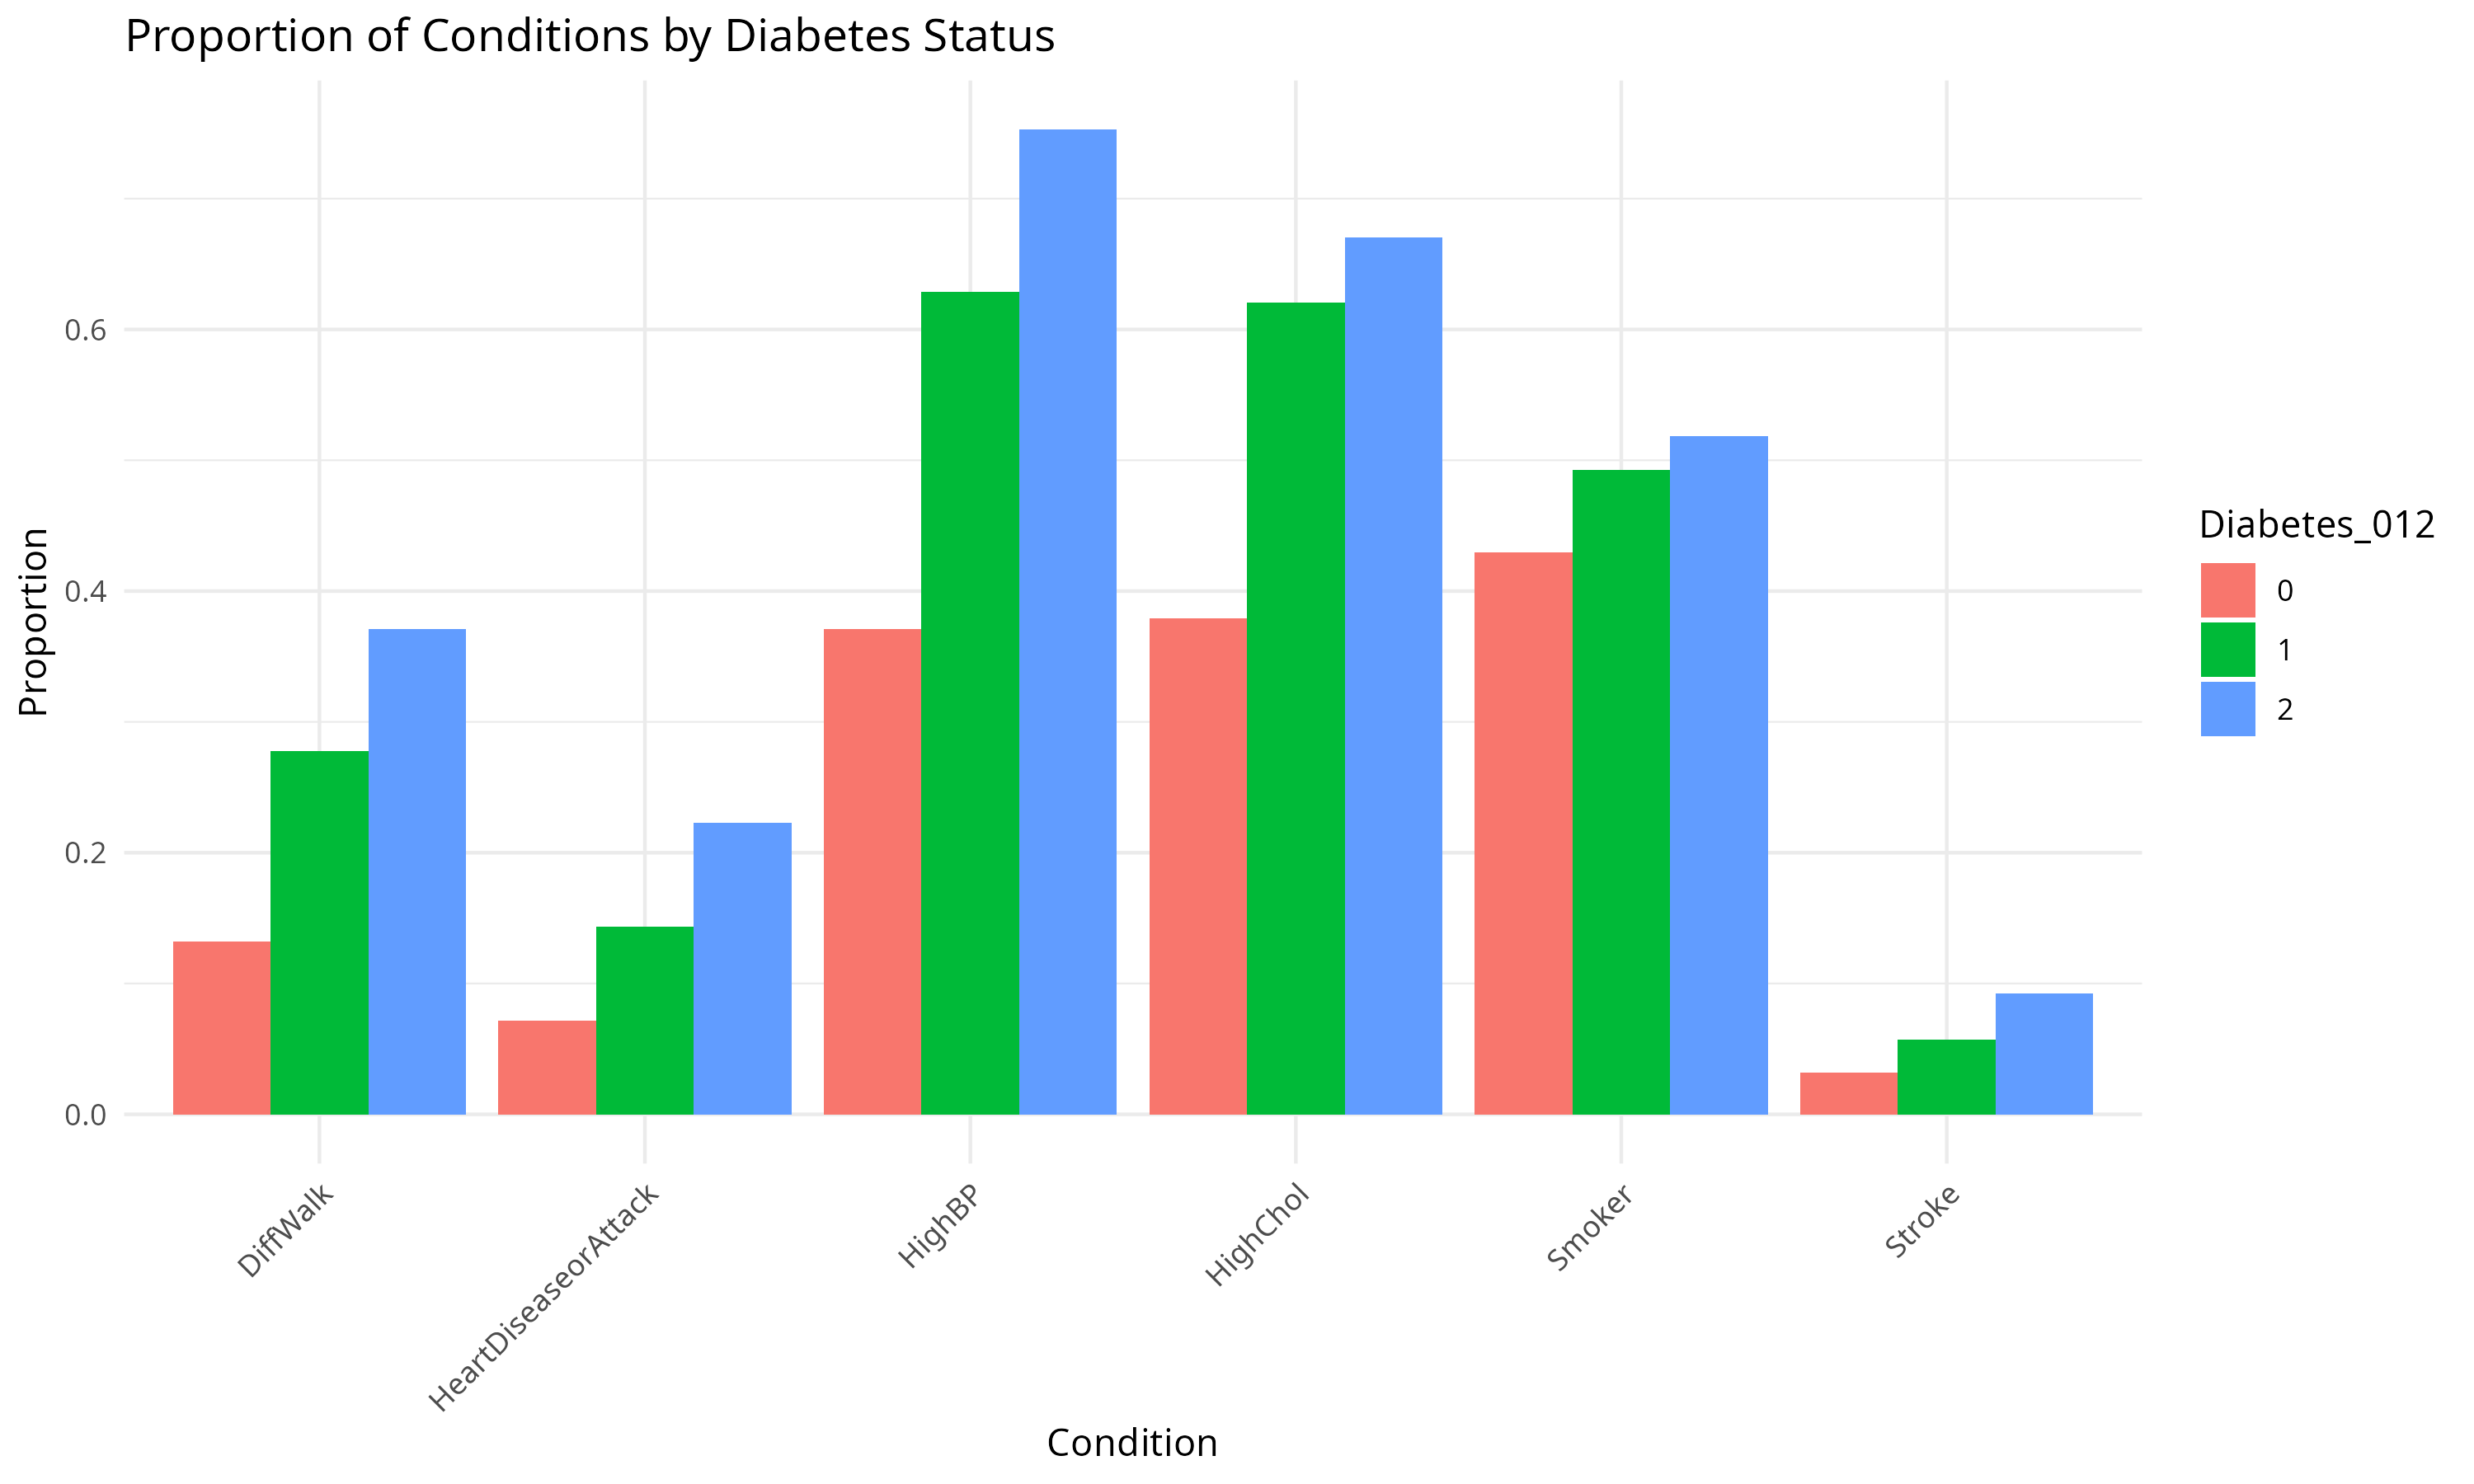
\includegraphics[width=1.0\textwidth]{outputs/figures/F3_prop_6vars.png}
    \caption{Tỷ lệ mắc các bệnh nền/thói quen xấu}
\end{figure}

Sự tương quan giữa các biến số (Spearman Correlation):
\begin{figure}[H]
    \centering
    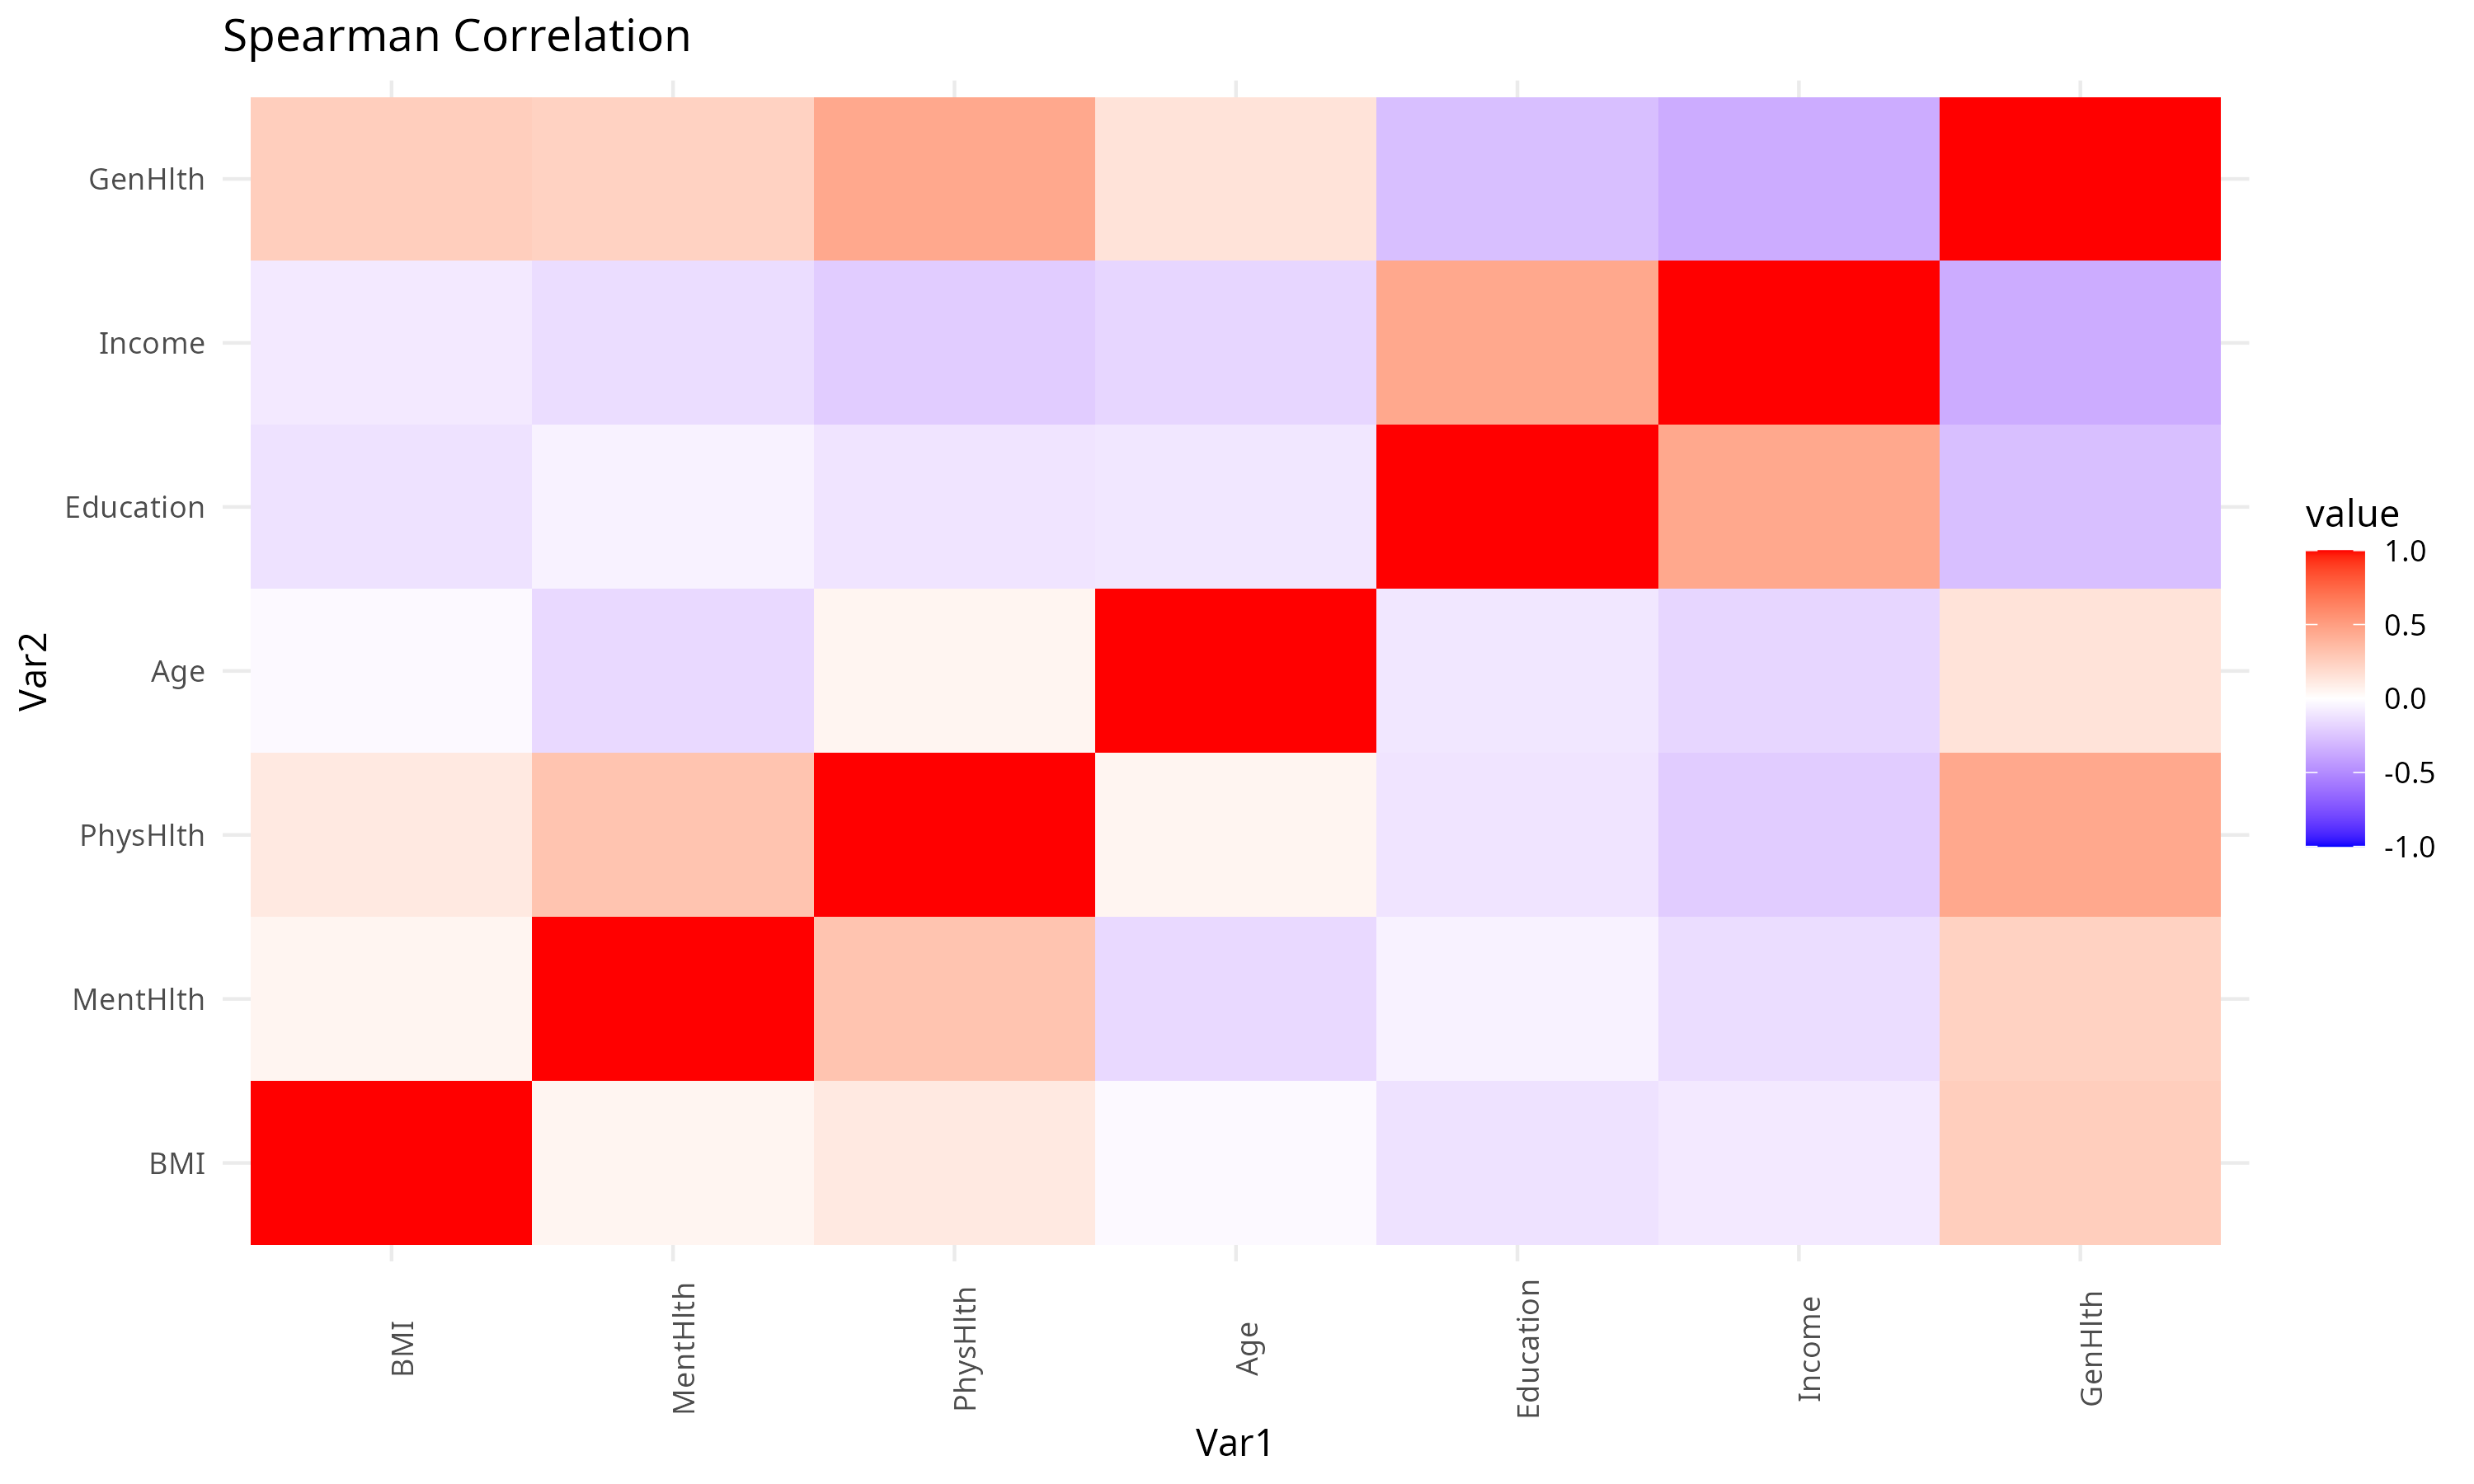
\includegraphics[width=0.7\textwidth]{outputs/figures/F5_spearman_corr.png}
    \caption{Ma trận tương quan Spearman}
\end{figure}

\subsection{5. Phân tích để đạt được mục tiêu}

\subsubsection{Phân tích thống kê (M2)}
Để xác định các yếu tố liên quan nhất, các kiểm định thống kê (Chi-square cho biến định danh và Kruskal-Wallis cho biến định lượng) đã được thực hiện. Kết quả xếp hạng dựa trên độ lớn ảnh hưởng (Effect Size - Cramer's V) cho thấy:
\begin{itemize}
    \item \textbf{Huyết áp cao (HighBP)} có mối liên hệ mạnh nhất với bệnh tiểu đường (Cramer's V = 0.27).
    \item Các yếu tố tiếp theo bao gồm \textbf{Khó khăn khi đi lại (DiffWalk, 0.22)}, \textbf{Sức khỏe chung (GenHlth, 0.22)}, và \textbf{Cholesterol cao (HighChol, 0.21)}.
    \item Chỉ số \textbf{BMI}, mặc dù là biến định lượng, cũng cho thấy sự khác biệt có ý nghĩa thống kê rất lớn giữa các nhóm (p-value $\approx$ 0).
\end{itemize}

\begin{table}[H]
    \centering
    \caption{Top 15 biến có ảnh hưởng lớn nhất}
    \resizebox{\textwidth}{!}{
        
\begin{tabular}{llrlrrrl}
\toprule
Variable & Test & p\_value & Effect\_Size\_Name & Effect\_Size\_Value & p\_adj\_fdr & p\_adj\_holm & Significant\\
\midrule
HighBP & Chi-square & 0 & Cramers\_V & 0.2721911 & 0 & 0 & TRUE\\
DiffWalk & Chi-square & 0 & Cramers\_V & 0.2244245 & 0 & 0 & TRUE\\
GenHlth & Chi-square & 0 & Cramers\_V & 0.2186154 & 0 & 0 & TRUE\\
HighChol & Chi-square & 0 & Cramers\_V & 0.2106712 & 0 & 0 & TRUE\\
HeartDiseaseorAttack & Chi-square & 0 & Cramers\_V & 0.1802807 & 0 & 0 & TRUE\\
\addlinespace
Age & Chi-square & 0 & Cramers\_V & 0.1378515 & 0 & 0 & TRUE\\
Income & Chi-square & 0 & Cramers\_V & 0.1241215 & 0 & 0 & TRUE\\
PhysActivity & Chi-square & 0 & Cramers\_V & 0.1222184 & 0 & 0 & TRUE\\
Stroke & Chi-square & 0 & Cramers\_V & 0.1072276 & 0 & 0 & TRUE\\
Education & Chi-square & 0 & Cramers\_V & 0.0948101 & 0 & 0 & TRUE\\
\addlinespace
CholCheck & Chi-square & 0 & Cramers\_V & 0.0680212 & 0 & 0 & TRUE\\
Smoker & Chi-square & 0 & Cramers\_V & 0.0631143 & 0 & 0 & TRUE\\
Veggies & Chi-square & 0 & Cramers\_V & 0.0593591 & 0 & 0 & TRUE\\
HvyAlcoholConsump & Chi-square & 0 & Cramers\_V & 0.0578961 & 0 & 0 & TRUE\\
BMI & Kruskal-Wallis & 0 & Epsilon\_Sq & 0.0557033 & 0 & 0 & TRUE\\
\bottomrule
\end{tabular}

    }
\end{table}

Ngoài ra, Permutation Test cũng được thực hiện để kiểm chứng sự khác biệt của BMI và Huyết áp cao. Kết quả cho thấy sự khác biệt là có ý nghĩa thống kê ($p$-value rất nhỏ).

\begin{figure}[H]
    \centering
    \begin{minipage}{0.48\textwidth}
        \centering
        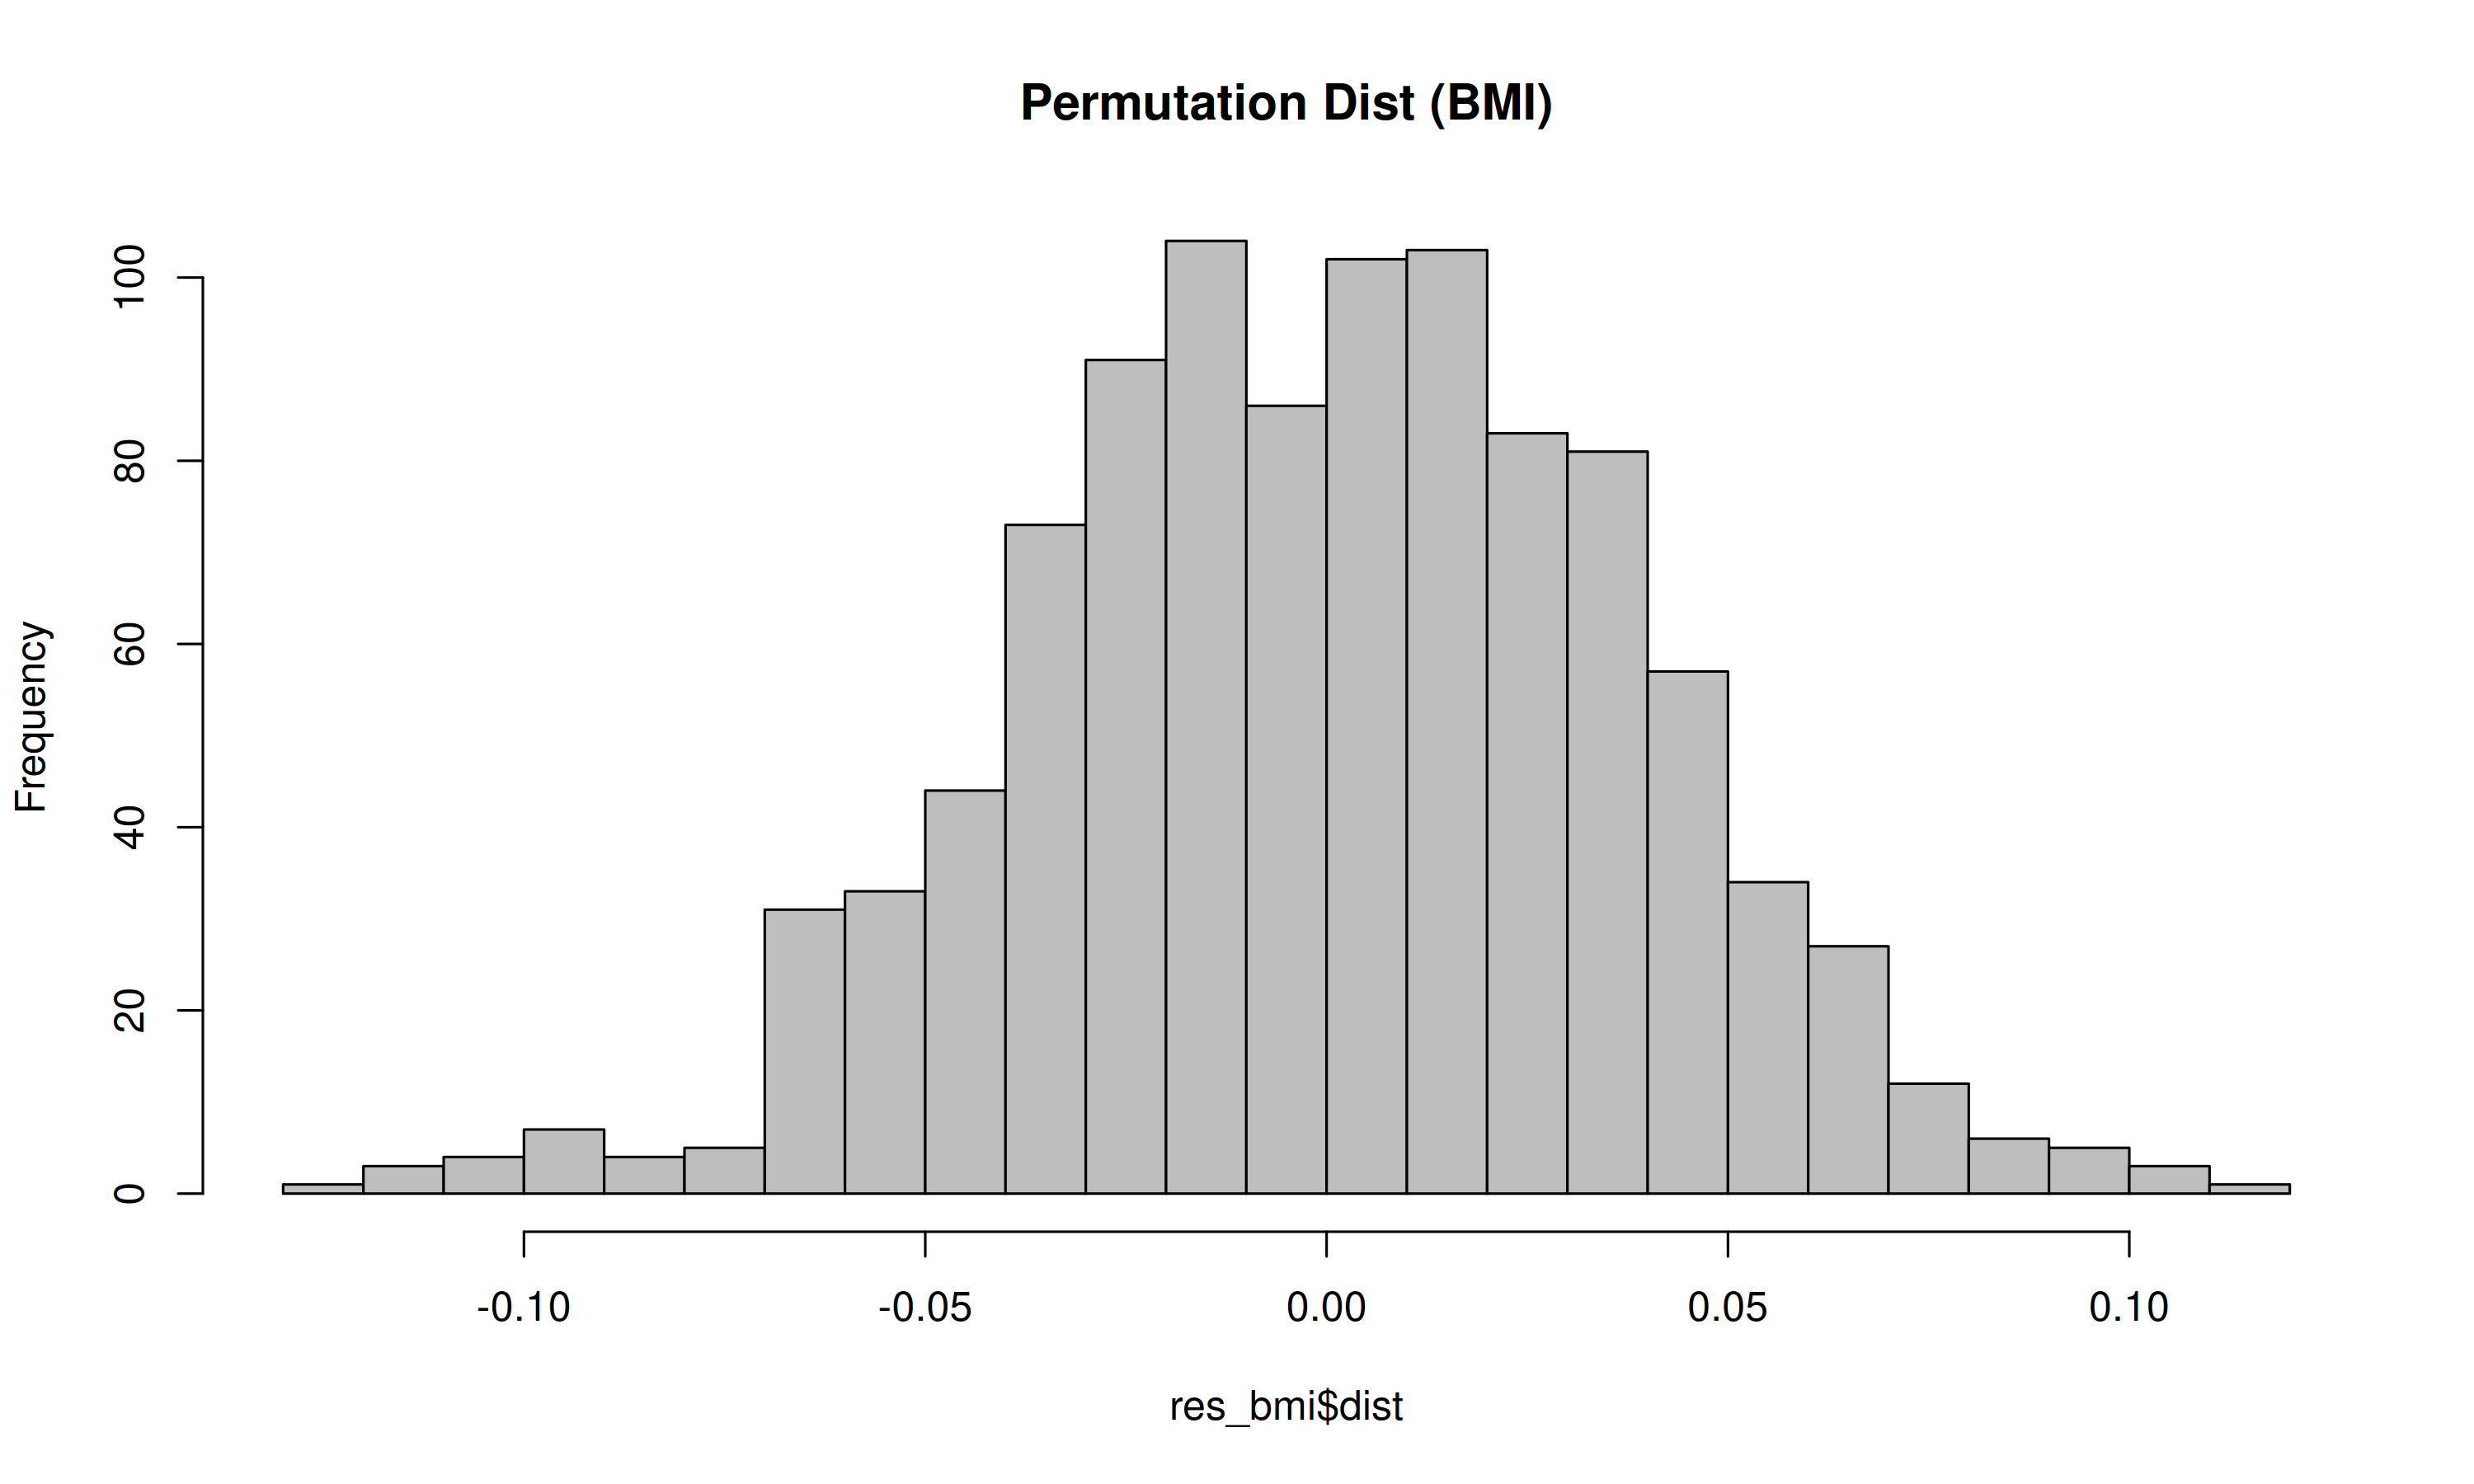
\includegraphics[width=\linewidth]{outputs/figures/F6_perm_bmi_diff.png}
        \caption{Permutation Test (BMI)}
    \end{minipage}\hfill
    \begin{minipage}{0.48\textwidth}
        \centering
        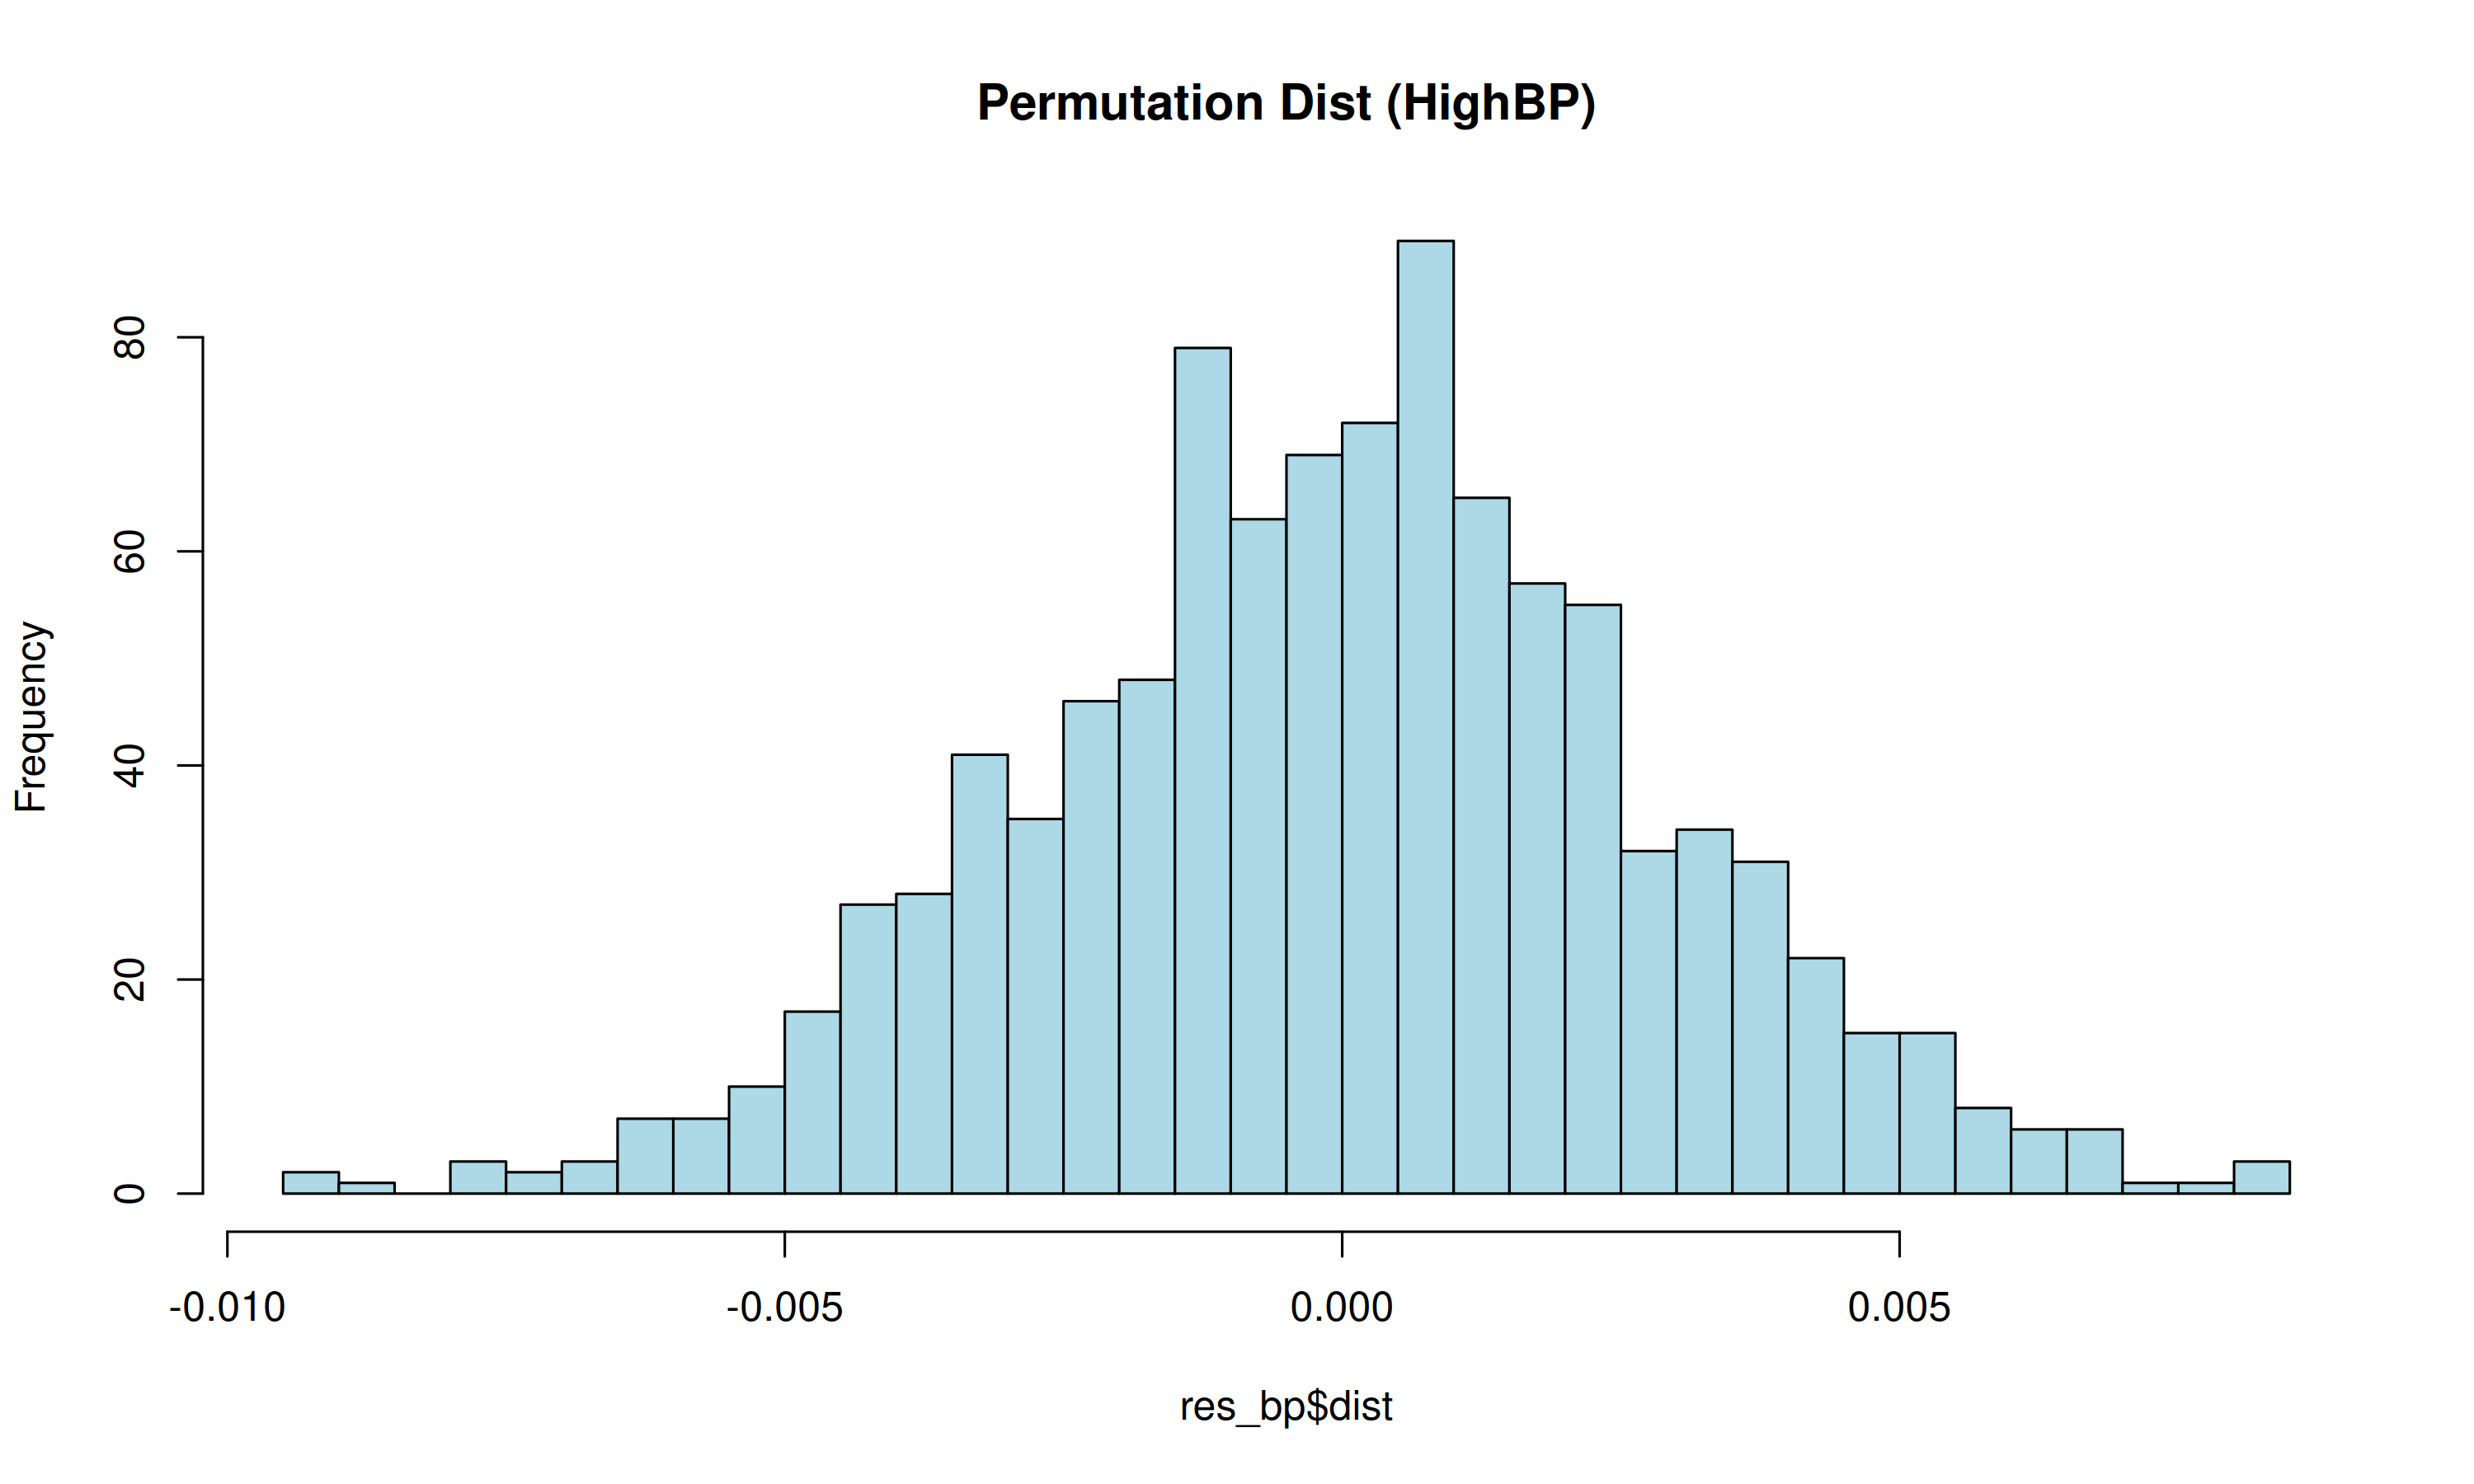
\includegraphics[width=\linewidth]{outputs/figures/F7_perm_highbp_diff.png}
        \caption{Permutation Test (HighBP)}
    \end{minipage}
\end{figure}

\subsubsection{Xây dựng và tối ưu mô hình (M3, M4)}
Quá trình huấn luyện bao gồm việc thử nghiệm nhiều thuật toán (Logistic Regression, LDA, QDA, Naive Bayes) kết hợp với các chiến lược xử lý mất cân bằng (None, Class Weight, Random Under-sampling).

Kết quả Grid Search (Bảng \ref{tab:gridsearch}) cho thấy sự đánh đổi rõ rệt giữa các chỉ số:
\begin{itemize}
    \item Với \textbf{Case A (3 lớp)}, do lớp "Tiền tiểu đường" quá nhỏ (1.8\%), hầu hết các mô hình đều gặp khó khăn. Mô hình LDA (chiến lược None) đạt kết quả F1 tốt nhất (~0.61) nhưng thực tế chủ yếu dự đoán đúng lớp đa số.
    \item Với \textbf{Case B (Tiểu đường vs Không)}, chiến lược \textbf{Random Under-sampling} giúp cân bằng lại dữ liệu, đưa \textbf{Naive Bayes} lên vị trí dẫn đầu về chỉ số F1 (~0.66). Nếu xét về độ cân bằng (Balanced Accuracy), \textbf{Logistic Regression (GLM) + Class Weight} lại vượt trội (0.74).
\end{itemize}

\begin{table}[H]
    \centering
    \caption{Kết quả Grid Search các mô hình}
    \label{tab:gridsearch}
    
\begin{tabular}{lllrrl}
\toprule
Case & Model & Strategy & CV\_F1 & CV\_BalAcc & CV\_AUC\\
\midrule
CaseA & multinom & None & 0.5904157 & NA & NA\\
CaseA & multinom & ClassWeight & 0.4267031 & NA & NA\\
CaseA & multinom & RandomUnderSampler & 0.4251965 & NA & NA\\
CaseA & nb & None & 0.4313275 & NA & NA\\
CaseA & nb & RandomUnderSampler & 0.4825447 & NA & NA\\
\addlinespace
CaseA & lda & None & 0.6111086 & NA & NA\\
CaseA & lda & RandomUnderSampler & 0.4204870 & NA & NA\\
CaseA & qda & None & 0.4258065 & NA & NA\\
CaseA & qda & RandomUnderSampler & 0.4088943 & NA & NA\\
CaseB & glm & None & 0.5826609 & 0.5666061 & NA\\
\addlinespace
CaseB & glm & ClassWeight & 0.6331140 & 0.7459898 & NA\\
CaseB & glm & RandomUnderSampler & 0.6327845 & 0.7457876 & NA\\
CaseB & nb & None & 0.6355811 & 0.6875599 & NA\\
CaseB & nb & RandomUnderSampler & 0.6575612 & 0.6820405 & NA\\
CaseB & lda & None & 0.6068428 & 0.5857391 & NA\\
\addlinespace
CaseB & lda & RandomUnderSampler & 0.6288254 & 0.7458555 & NA\\
CaseB & qda & None & 0.6302141 & 0.6804052 & NA\\
CaseB & qda & RandomUnderSampler & 0.5977686 & 0.7250941 & NA\\
CaseC & glm & None & 0.5954110 & 0.5779638 & NA\\
CaseC & glm & ClassWeight & 0.6434991 & 0.7417341 & NA\\
\addlinespace
CaseC & glm & RandomUnderSampler & 0.6435145 & 0.7416772 & NA\\
CaseC & nb & None & 0.6430327 & 0.6838693 & NA\\
CaseC & nb & RandomUnderSampler & 0.6626470 & 0.6719265 & NA\\
CaseC & lda & None & 0.6138271 & 0.5932228 & NA\\
CaseC & lda & RandomUnderSampler & 0.6400972 & 0.7414865 & NA\\
\addlinespace
CaseC & qda & None & 0.6357973 & 0.6749288 & NA\\
CaseC & qda & RandomUnderSampler & 0.6135700 & 0.7177495 & NA\\
\bottomrule
\end{tabular}

\end{table}

Tổng hợp lại, các mô hình tốt nhất được lựa chọn cho từng bài toán như sau:

\begin{table}[H]
    \centering
    \caption{Mô hình tốt nhất cho từng Case}
    \resizebox{\textwidth}{!}{
        
\begin{tabular}{lllrrlr}
\toprule
Case & Model & Strategy & CV\_F1 & CV\_BalAcc & CV\_AUC & Test\_F1\\
\midrule
CaseA & lda & None & 0.6111086 & NA & NA & 0.6083774\\
CaseB & nb & RandomUnderSampler & 0.6575612 & 0.6820405 & NA & 0.6609283\\
CaseC & nb & RandomUnderSampler & 0.6626470 & 0.6719265 & NA & 0.6664380\\
\bottomrule
\end{tabular}

    }
\end{table}

Chi tiết hiệu năng của mô hình tốt nhất (Confusion Matrix và ROC):

\begin{figure}[H]
    \centering
    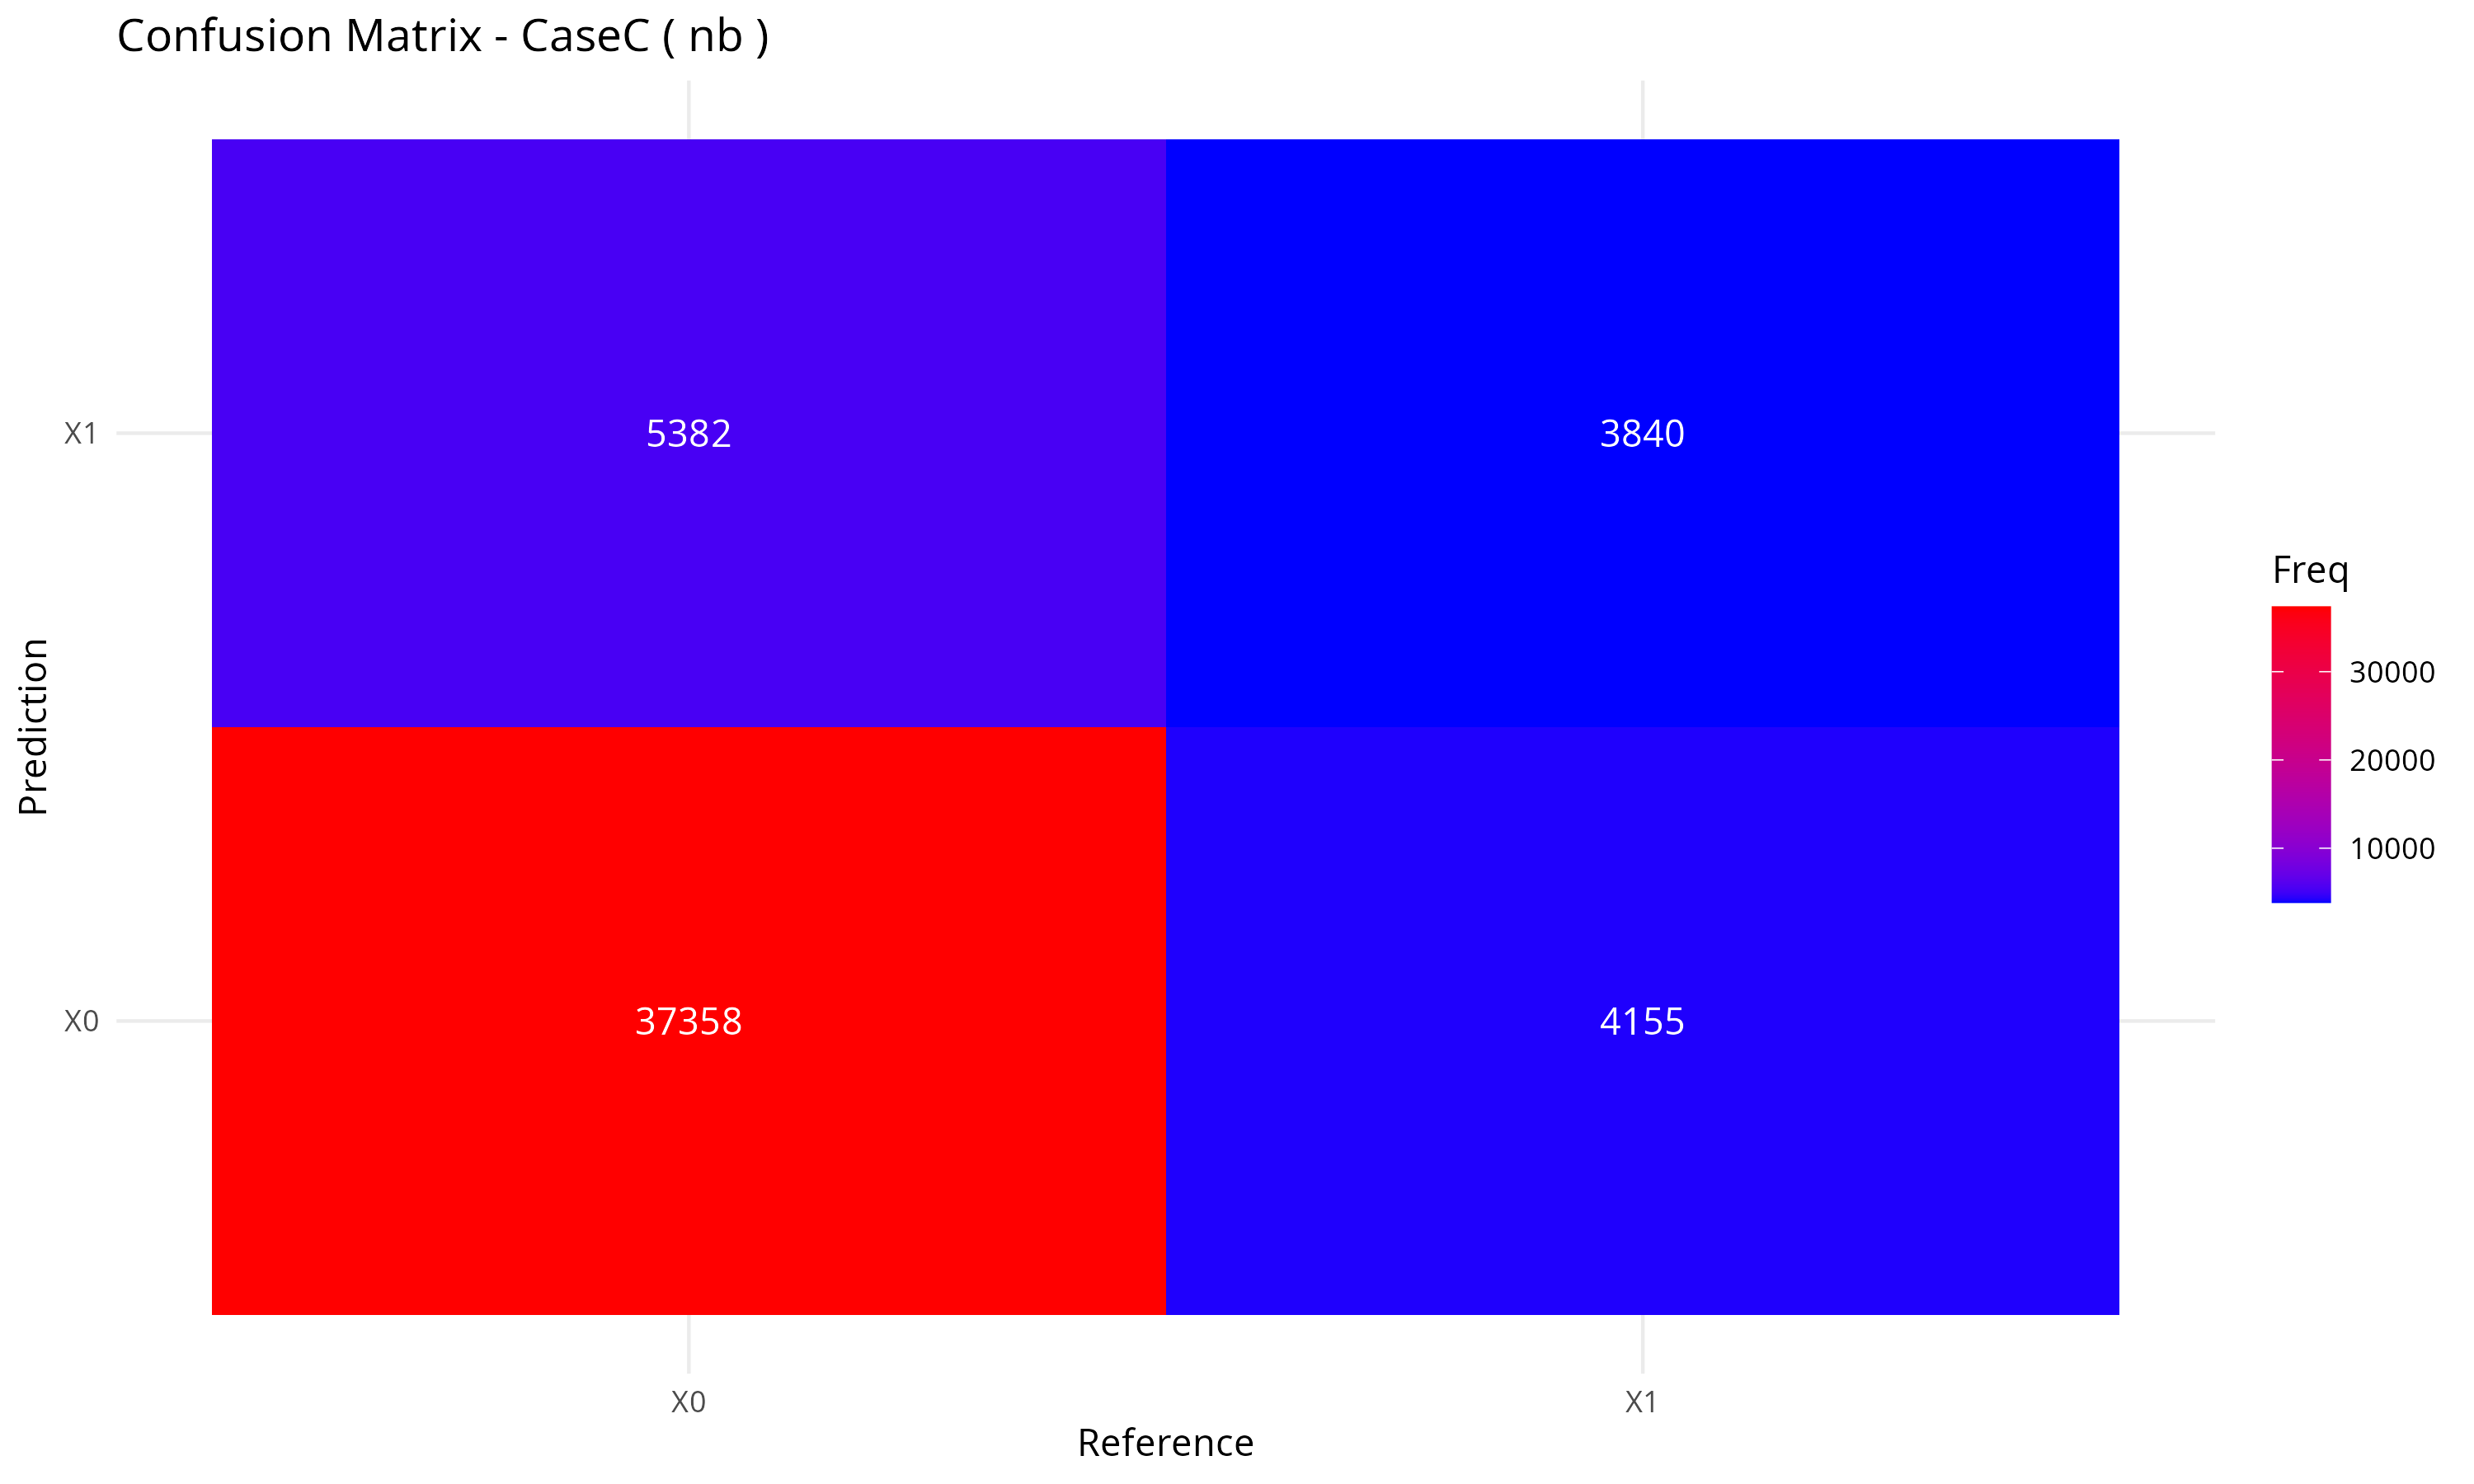
\includegraphics[width=0.6\textwidth]{outputs/figures/F8_confusion_bestcase.png}
    \caption{Confusion Matrix của mô hình tốt nhất}
\end{figure}

\begin{figure}[H]
    \centering
    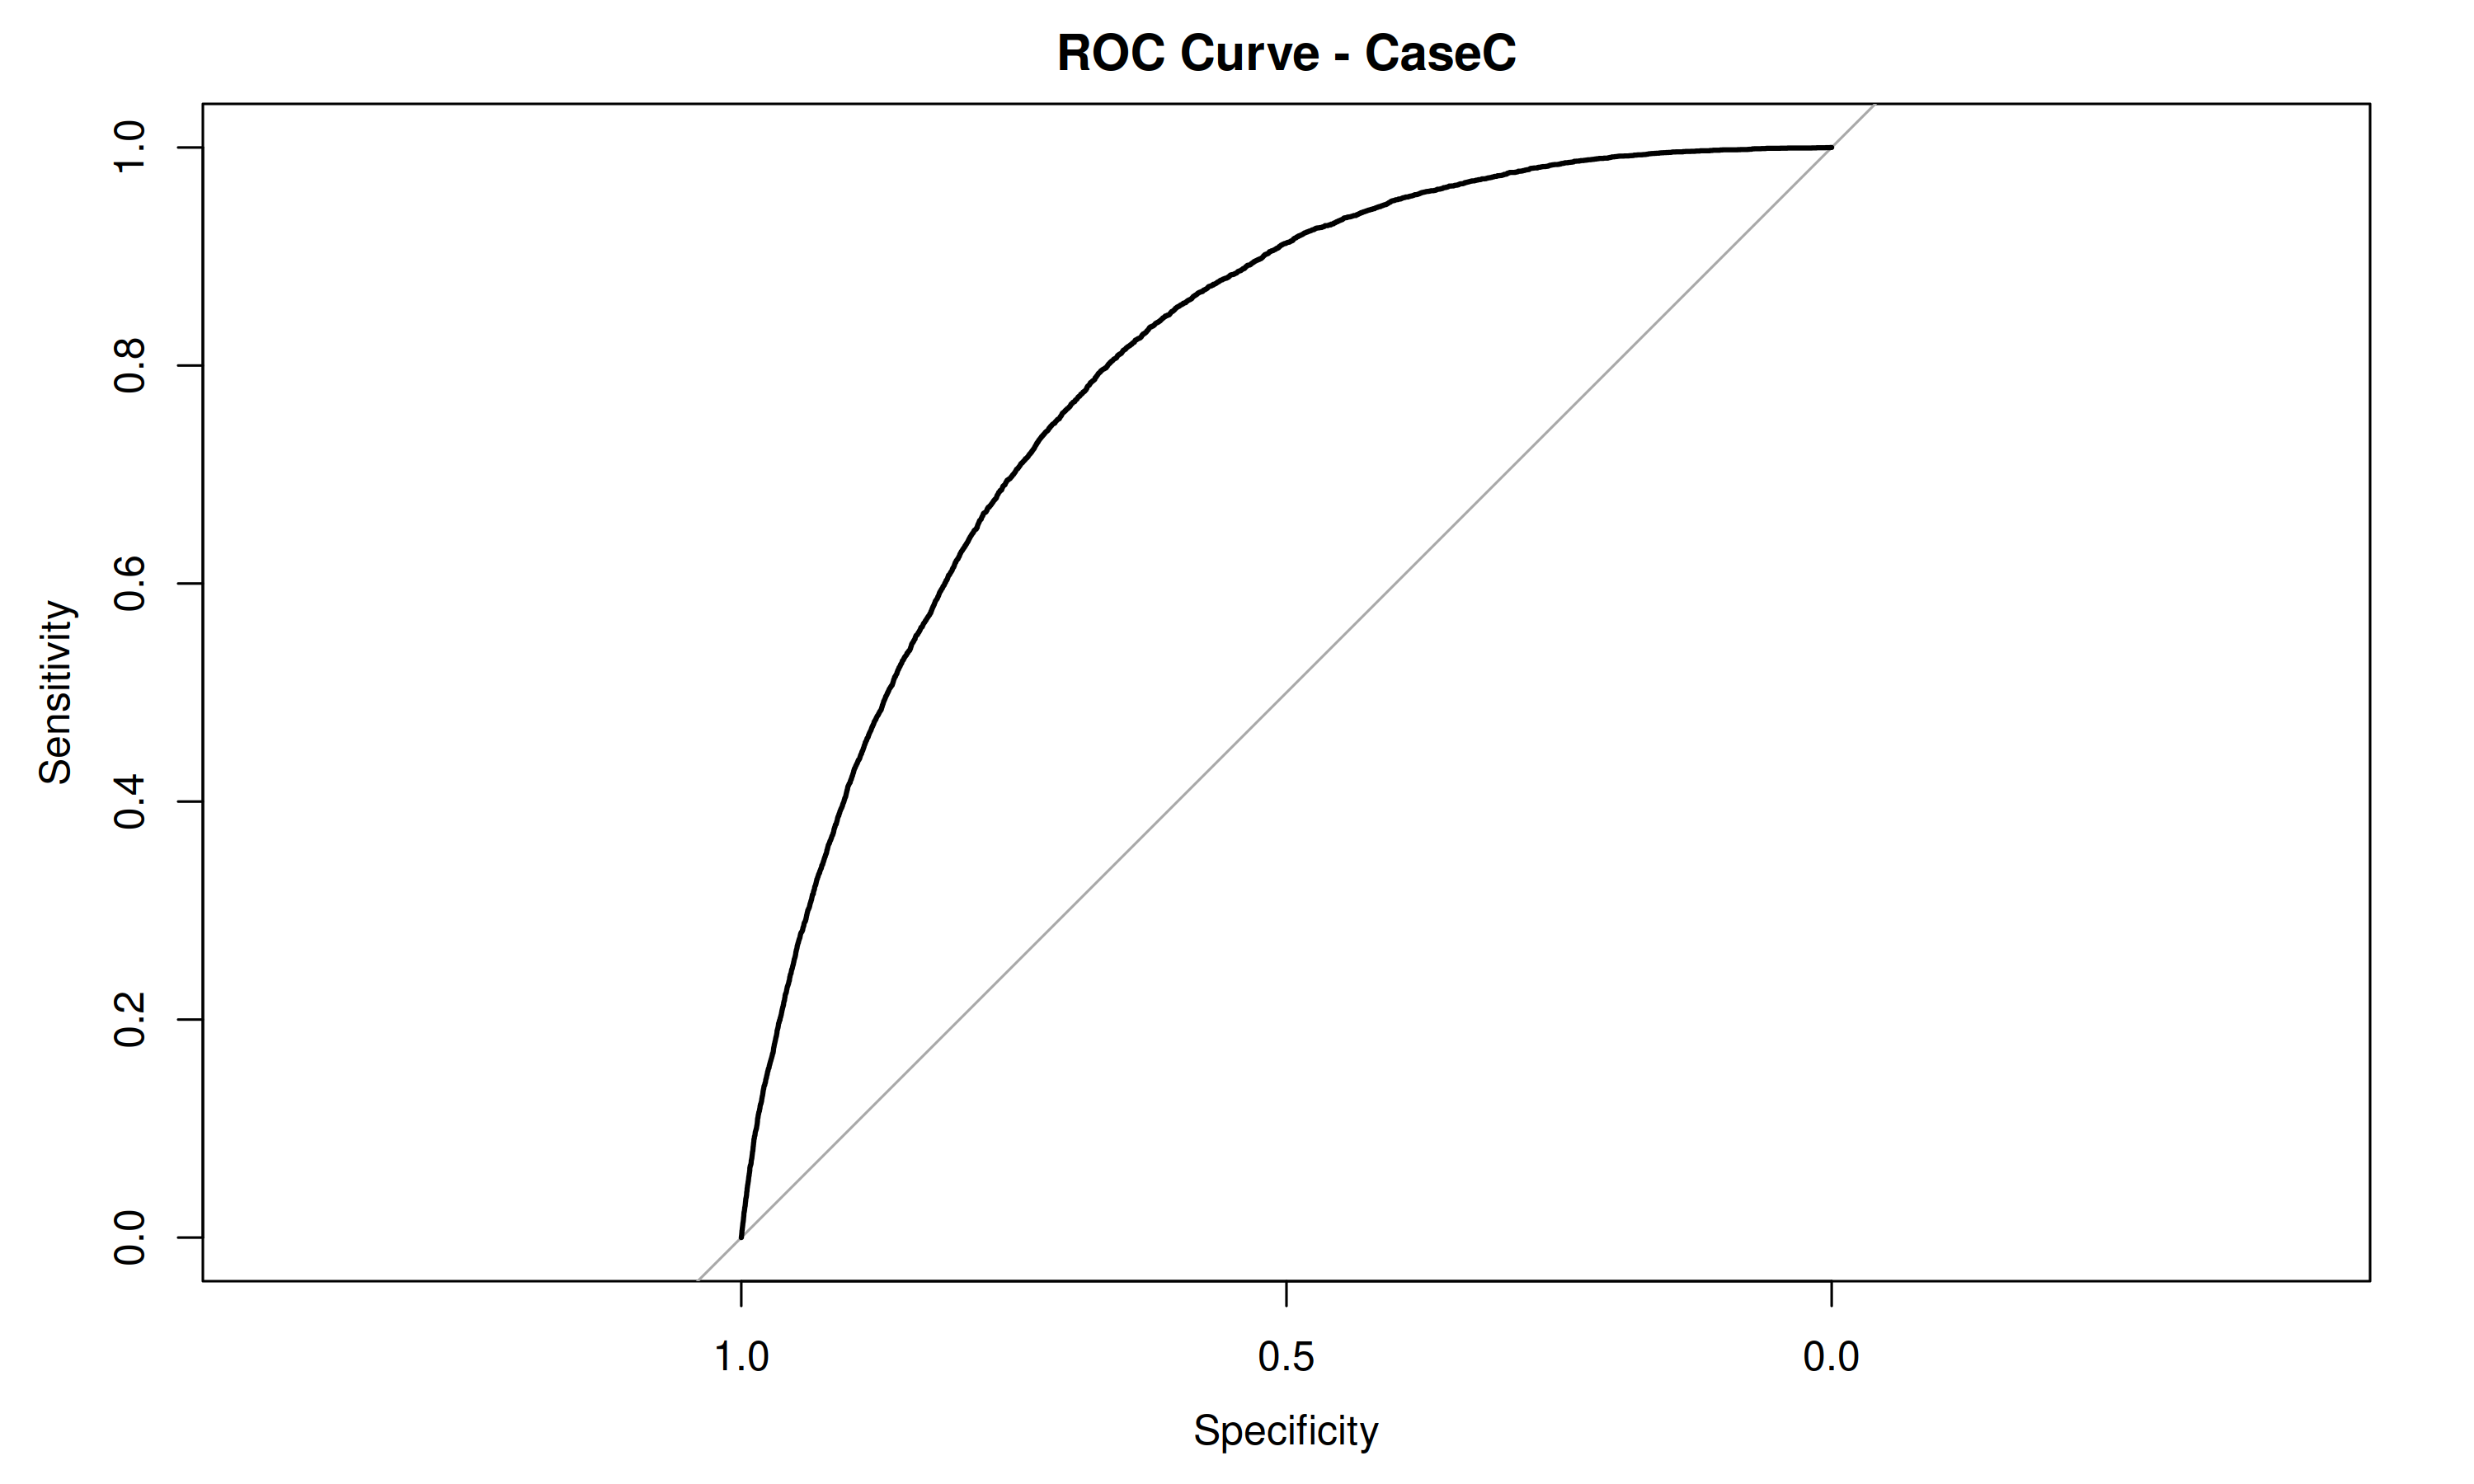
\includegraphics[width=0.6\textwidth]{outputs/figures/F9_roc_bestcase.png}
    \caption{Đường cong ROC}
\end{figure}

\subsection{6. Nhận xét và kết luận}
Qua quá trình phân tích dữ liệu và xây dựng mô hình, các kết luận chính được rút ra như sau:

\begin{itemize}
    \item \textbf{Mất cân bằng dữ liệu là thách thức lớn nhất:} Với tỷ lệ mất cân bằng lên tới 46:1 ở Case A, việc dự đoán chính xác nhóm "Tiền tiểu đường" là cực kỳ khó khăn nếu chỉ dùng các biến khảo sát thông thường. Các mô hình có xu hướng dự đoán nghiêng về nhóm đa số (Khỏe mạnh).
    \item \textbf{Vai trò của các chỉ số sức khỏe:} Phân tích thống kê đã định lượng rõ ràng mức độ ảnh hưởng của \textbf{Huyết áp cao (HighBP)}, \textbf{Khó khăn vận động (DiffWalk)} và \textbf{BMI}. Những người có BMI > 30 và tiền sử huyết áp cao có nguy cơ mắc bệnh cao gấp nhiều lần.
    \item \textbf{Hiệu quả của các chiến lược xử lý:}
          \begin{itemize}
              \item \textbf{Random Under-sampling} đã chứng minh hiệu quả vượt trội trong việc cải thiện F1-score cho bài toán nhị phân, giúp mô hình Naive Bayes đạt độ ổn định tốt nhất.
              \item \textbf{Class Weight} là lựa chọn thay thế tốt nếu mục tiêu là tối đa hóa Balanced Accuracy mà không muốn bỏ bớt dữ liệu huấn luyện.
          \end{itemize}
    \item \textbf{Khuyến nghị thực tế:} Mô hình xây dựng được có giá trị cao trong việc \textbf{sàng lọc ban đầu} (screening). Với khả năng nhận diện tốt các nhóm nguy cơ cao (dựa trên Recall/Sensitivity được cải thiện nhờ Under-sampling), hệ thống có thể cảnh báo sớm cho người dùng để họ chủ động thực hiện các xét nghiệm y tế chuyên sâu hơn.
\end{itemize}

\newpage
\begin{thebibliography}{8}
    \bibitem{brfss}
    CDC, "Behavioral Risk Factor Surveillance System (BRFSS) 2015 Codebook Report," \emph{Centers for Disease Control and Prevention}, 2015.
    \bibitem{sklearn}
    Pedregosa et al., "Scikit-learn: Machine Learning in Python," \emph{JMLR 12}, pp. 2825-2830, 2011.
    \bibitem{caret}
    Kuhn, M., "Building Predictive Models in R Using the caret Package," \emph{Journal of Statistical Software}, 28(5), 1-26, 2008.
\end{thebibliography}

\end{document}